\chapter{Outils pour la robotique reproductible}\label{ch:ducker}

\setlength{\epigraphwidth}{0.93\textwidth}
\epigraph{La seule façon de réaliser des progrès substantiels dans un domaine quelconque est de s'appuyer sur le travail des autres. Pourtant, la programmation informatique reste une industrie artisanale car les programmeurs insistent pour réinventer des programmes pour chaque nouvelle application, au lieu d'utiliser ce qui existe déjà. Nous devons encourager une manière de regrouper les programmes de manière à ce qu'ils puissent être perçus comme des outils standard, chacun accomplissant sa tâche spécialisée suffisamment bien et s'interfacant avec d'autres outils de manière si pratique que les programmeurs ressentent rarement le besoin de créer leur propre version à partir de zéro.''}{\begin{flushright}--\citet{kernighan1976software}, \href{https://dl.acm.org/doi/10.1145/1010726.1010728}{\textit{Software tools}}\end{flushright}}

Dans ce chapitre, nous abordons le défi de la reproductibilité des logiciels et la manière dont les meilleures pratiques du génie logiciel, telles que les outils d'intégration continue et de conteneurisation, peuvent aider les chercheurs à atténuer la variabilité associée à la construction et à la maintenance des logiciels de robotique. D'une manière générale, nos travaux tentent d'isoler les sources de variabilité computationnelle, et n'envisagent pas les notions de variabilité statistique découlant de l'incertitude aléatoire ou épistémique~\citep{diaz2018interactive}. Cependant, la réduction de la variabilité informatique (qui entrave souvent la reproductibilité expérimentale) est une étape clé pour permettre aux chercheurs d'identifier et de diagnostiquer plus rapidement ces variables plus insaisissables en robotique et en apprentissage machine.

Afin d'aborder la question de la reproductibilité des logiciels, nous avons rassemblé un ensemble d'outils et de flux de développement représentant les meilleures pratiques en matière de génie logiciel. Ces outils sont principalement basés sur la \textit{containerisation}, une technologie de virtualisation largement adoptée dans l'industrie du logiciel. Pour abaisser la barrière d'entrée pour les nouveaux contributeurs et minimiser la variabilité entre les plates-formes matérielles, nous avons développé une infrastructure de conteneurs de pointe basée sur Docker~\citep{merkel2014docker}, un moteur de conteneurs très populaire. Docker permet aux utilisateurs de mettre en place des artefacts de déploiement versionnés qui figent efficacement un système de fichiers entier, et de gérer les contraintes de ressources via un environnement d'exécution en "sandboxed".

Le contenu de ce chapitre est organisé comme suit. Dans \autoref{sec:dependency-management} nous introduisons le problème de la résolution des dépendances et le défi de la construction d'artefacts logiciels reproductibles. Dans \autoref{sec:os-and-virtualization}, nous décrivons une solution générale à ce problème, la virtualisation des logiciels. Ensuite, dans \autoref{sec:containerization}, nous discutons d'une approche légère de la virtualisation, connue sous le nom de conteneurisation. Dans \autoref{sec:docker-intro}, nous faisons une visite guidée à travers une implémentation de conteneur, appelée Docker. Enfin, dans \autoref{sec:ros-docker}, nous présentons DuckieOS, un environnement dockerisé pour la construction d'applications robotiques reproductibles pour la recherche et l'utilisation pédagogique.

\section{Dependency management}\label{sec:dependency-management}

Une source commune de variabilité dans le développement de logiciels est la dépendance des logiciels. Pendant de nombreuses années, les développeurs ont eu du mal à gérer les dépendances avant qu'on ne découvre que le problème de résolution des dépendances était NP-complete~\citep{abate2012dependency}. Si nous supposons qu'aucune version de la même dépendance ne peut être installée simultanément, alors pour un ensemble donné de logiciels qui doivent être installés, et de dépendances nécessaires pour les installer, la détermination de la version cohérente la plus récente des dépendances est aussi difficile que les problèmes les plus difficiles de NP. Officieusement, ce problème est connu sous le nom de \textit{dependency hell} et devient de plus en plus problématique à mesure que les projets logiciels se développent et introduisent de nouvelles dépendances.

L'enfer des dépendances ne se produit pas seulement à l'intérieur des projets logiciels individuels, mais aussi à travers les projets et les environnements de développement. Des centaines de gestionnaires de paquets ont été développés pour divers systèmes d'exploitation, langages de programmation et cadres de développement. Ubuntu dispose du \href{https://help.ubuntu.com/lts/serverguide/apt.html}{Advanced Package Tool} (\inline{apt}), macOS a \href{https://brew.sh/}{Homebrew} (\inline{brew}), Windows a \href{https://chocolatey.org/}{Chocolatey} (\inline{choco}). La plupart des écosystèmes de langage de programmation ont leurs propres gestionnaires de paquets sur mesure ; \href{https://conan.io/}{Conan} pour C/C++, \href{https://maven.apache.org}{Maven} pour Java, et \href{https://www.haskell.org/cabal/}{Cabal} pour Haskell. Python a développé de nombreuses solutions qui se chevauchent pour la gestion des paquets, notamment \href{https://pypi.org/project/pip/}{pip}, \href{https://www.anaconda.com/}{Anaconda}, \href{https://github.com/pyenv/pyenv}{PyEnv}, \href{https://virtualenv.pypa.io/}{Virtualenv}, et d'autres. Certains d'entre eux installent des paquets pour l'ensemble du système, et d'autres fournissent des environnements en ligne de commande. Au cours de la vie d'un système informatique, à mesure que les paquets sont installés et partiellement supprimés, il devient difficile de suivre les changements et leurs effets secondaires.

Le problème provient essentiellement de l'exigence selon laquelle aucune version de la même dépendance ne peut être installée simultanément. En outre, les installateurs de logiciels ont tendance à pulvériser des fichiers dans le système de fichiers, qui peuvent être corrompus et sont difficiles à supprimer complètement si le besoin s'en fait sentir. Pour résoudre ces problèmes, il faut une certaine notion de "contrôle", de sorte que lorsqu'un nouveau logiciel est installé, toute modification ultérieure puisse être retracée et annulée. Des sauvegardes matérielles feraient l'affaire, mais elles sont lourdes à gérer et ne conviennent pas à des fins de développement. Il serait plutôt pratique de disposer d'un outil permettant aux applications de créer un système de fichiers privé, d'installer leurs dépendances et d'éviter de contaminer le système d'exploitation hôte.

\section{Operating systems and virtualization}\label{sec:os-and-virtualization}

Avec la croissance des opérations de développement (devops), un certain nombre de solutions ont émergé pour la construction et l'exécution d'artefacts logiciels génériques. La plupart de ces solutions sont des émulateurs, qui simulent complètement une architecture de processeur étrangère, et donc tout logiciel qui s'exécute sur celle-ci. Une autre solution est celle des machines virtuelles (VM), une sorte d'environnement d'exécution isolé qui utilise un \textit{hypervisor} pour faciliter l'accès au matériel, mais qui fonctionne généralement sur du métal nu. L'inconvénient de ces deux méthodes est leur efficacité. Les machines virtuelles contiennent des systèmes d'exploitation à part entière et sont donc lourdes à exécuter et à déboguer. Cela est particulièrement inutile pour construire et exécuter une petite application sur un système d'exploitation étranger. Les émulateurs fonctionnent beaucoup plus lentement que le code machine natif, selon les architectures hôte et cible.

En 2006, Linux a introduit plusieurs nouvelles fonctionnalités du noyau pour contrôler des groupes de processus, sous l'égide de \textbf{cgroups}~\citep{menage2007adding}. Collectivement, ces fonctionnalités prennent en charge une forme de virtualisation légère, présentant de nombreux avantages des machines virtuelles (VM) tels que le contrôle des ressources et l'isolation de l'espace de noms, sans les surcharges de calcul associées à la virtualisation complète. Ces fonctionnalités ont ouvert la voie à un ensemble d'outils qui sont aujourd'hui connus sous le nom de conteneurs. Contrairement aux machines virtuelles, les conteneurs partagent un noyau commun, mais restent isolés de leur système d'exploitation hôte et des conteneurs frères et sœurs. Alors que les machines virtuelles nécessitent souvent du matériel de type serveur pour fonctionner correctement, les conteneurs conviennent à une catégorie beaucoup plus large de plateformes mobiles et embarquées en raison de leur faible empreinte sur les ressources.

\begin{figure}
\centrer
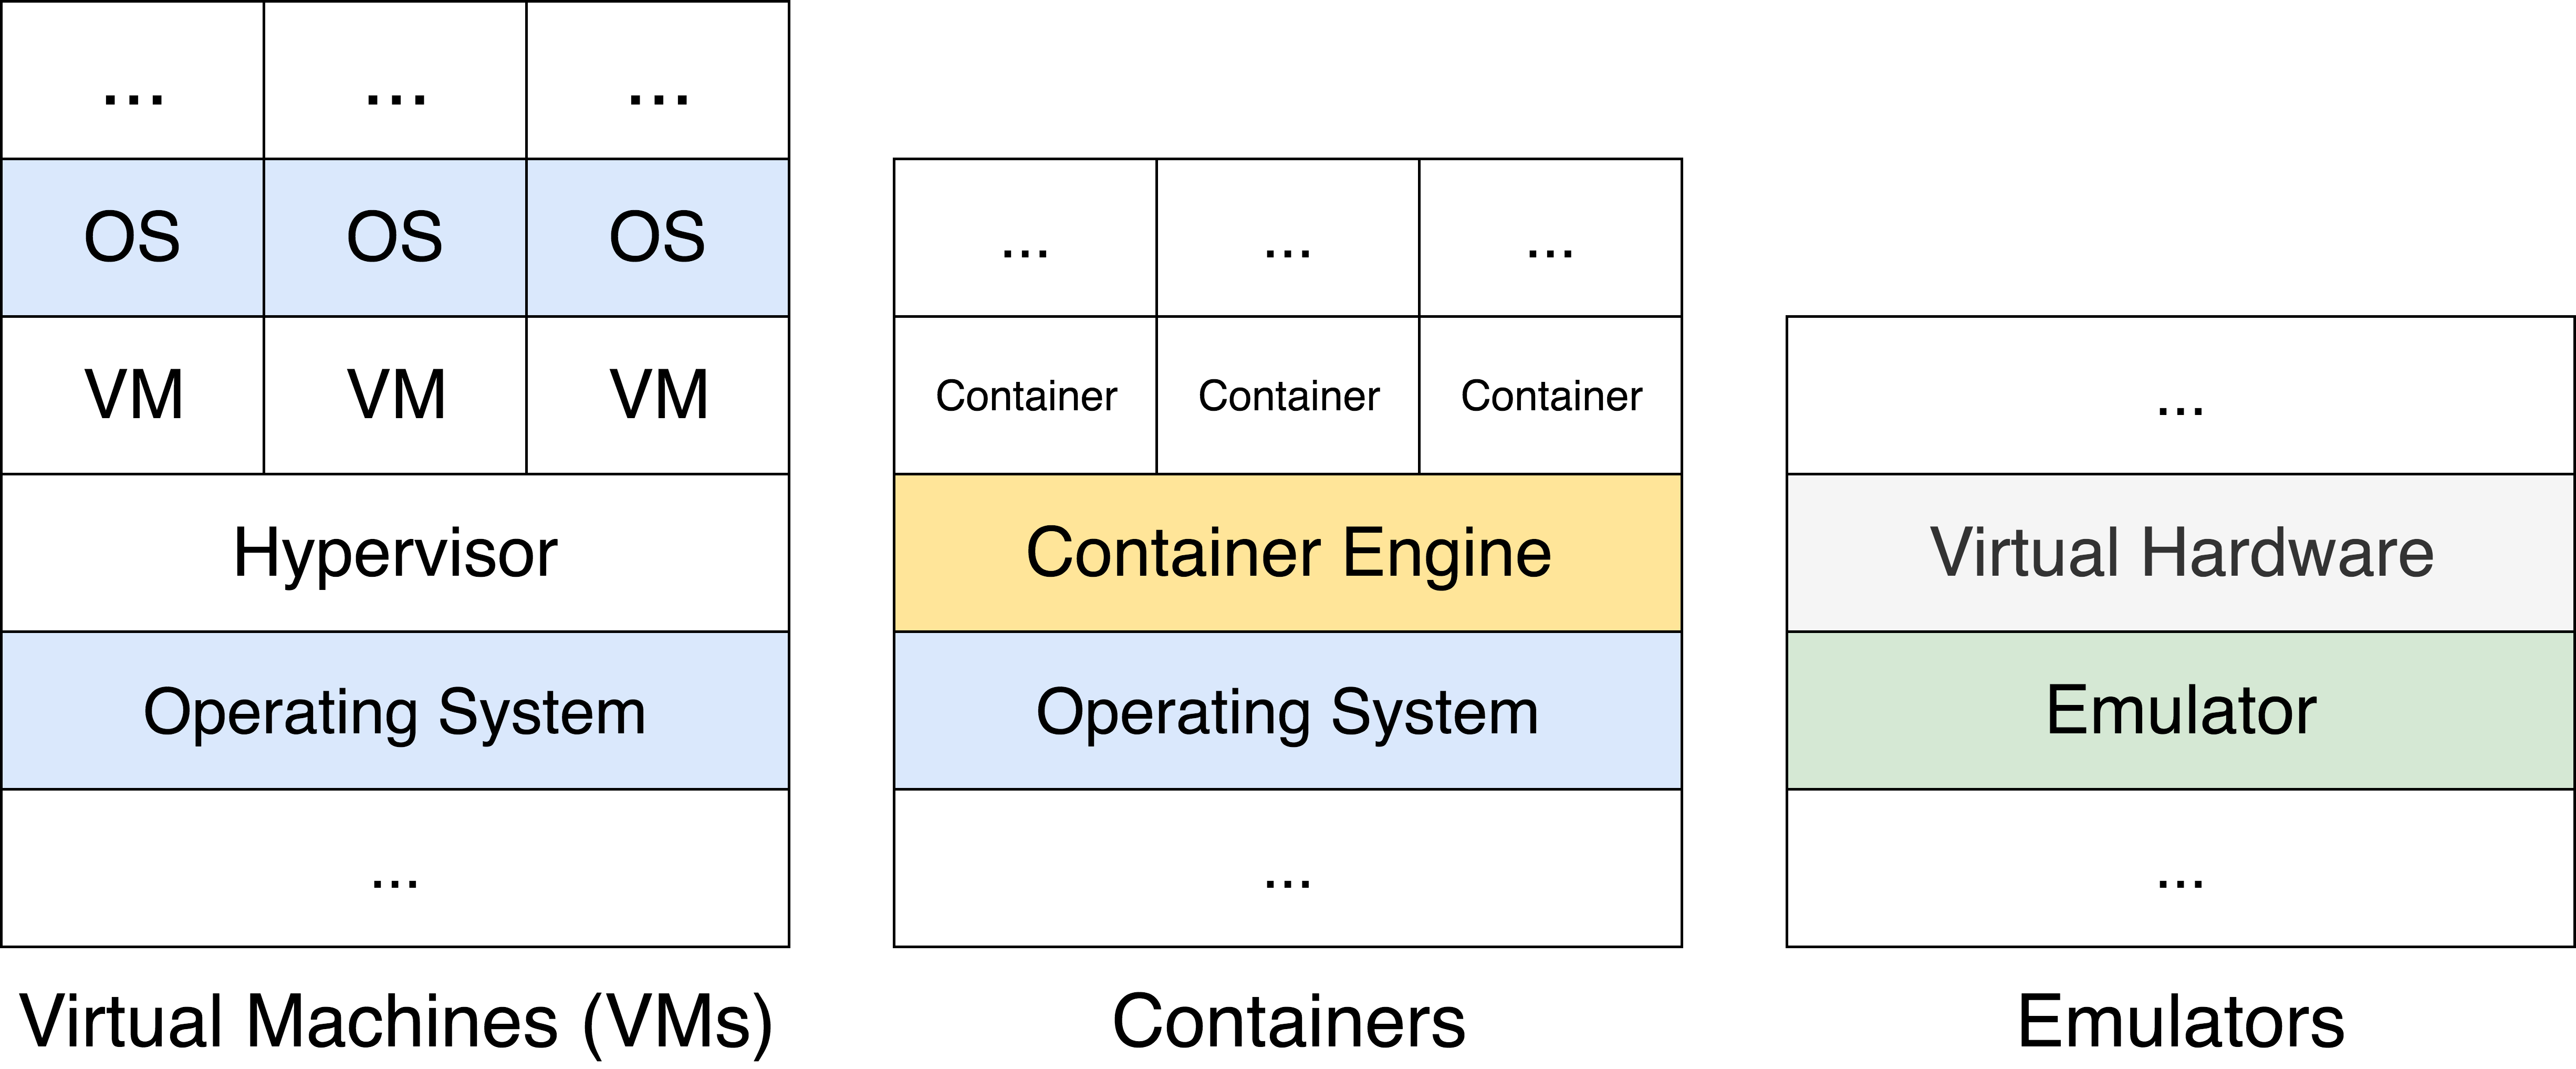
\includegraphics[width=0.70\textwidth]{../figures/vms_containers_emulators.png}
\caption{La virtualisation complète est un processus très gourmand en ressources. La conteneurisation est moins coûteuse, car elle partage un noyau avec le système d'exploitation hôte. L'émulation nous permet d'émuler le matériel comme un logiciel. Chacune de ces méthodes peut être utilisée en conjonction avec n'importe quelle autre.\vspace{-10pt}}
\label{fig:vms_containers_emulators}
\end{figure}

\section{Containerization}\label{sec:containerization}

L'un des défis du développement de logiciels distribués sur des plates-formes hétérogènes est le problème de la variabilité. L'accélération du rythme de développement des logiciels s'accompagne d'une charge supplémentaire de maintenance des logiciels. À mesure que les piles de matériel et de logiciels évoluent, le code source doit être périodiquement mis à jour pour être construit et fonctionner correctement. Maintenir une base de code stable et bien documentée peut représenter un défi considérable, en particulier dans un cadre universitaire où les contributeurs rejoignent et quittent fréquemment un projet. Ensemble, ces défis constituent des obstacles importants à la reproductibilité expérimentale et à la collaboration scientifique.

\begin{figure}[ht]
\centrer
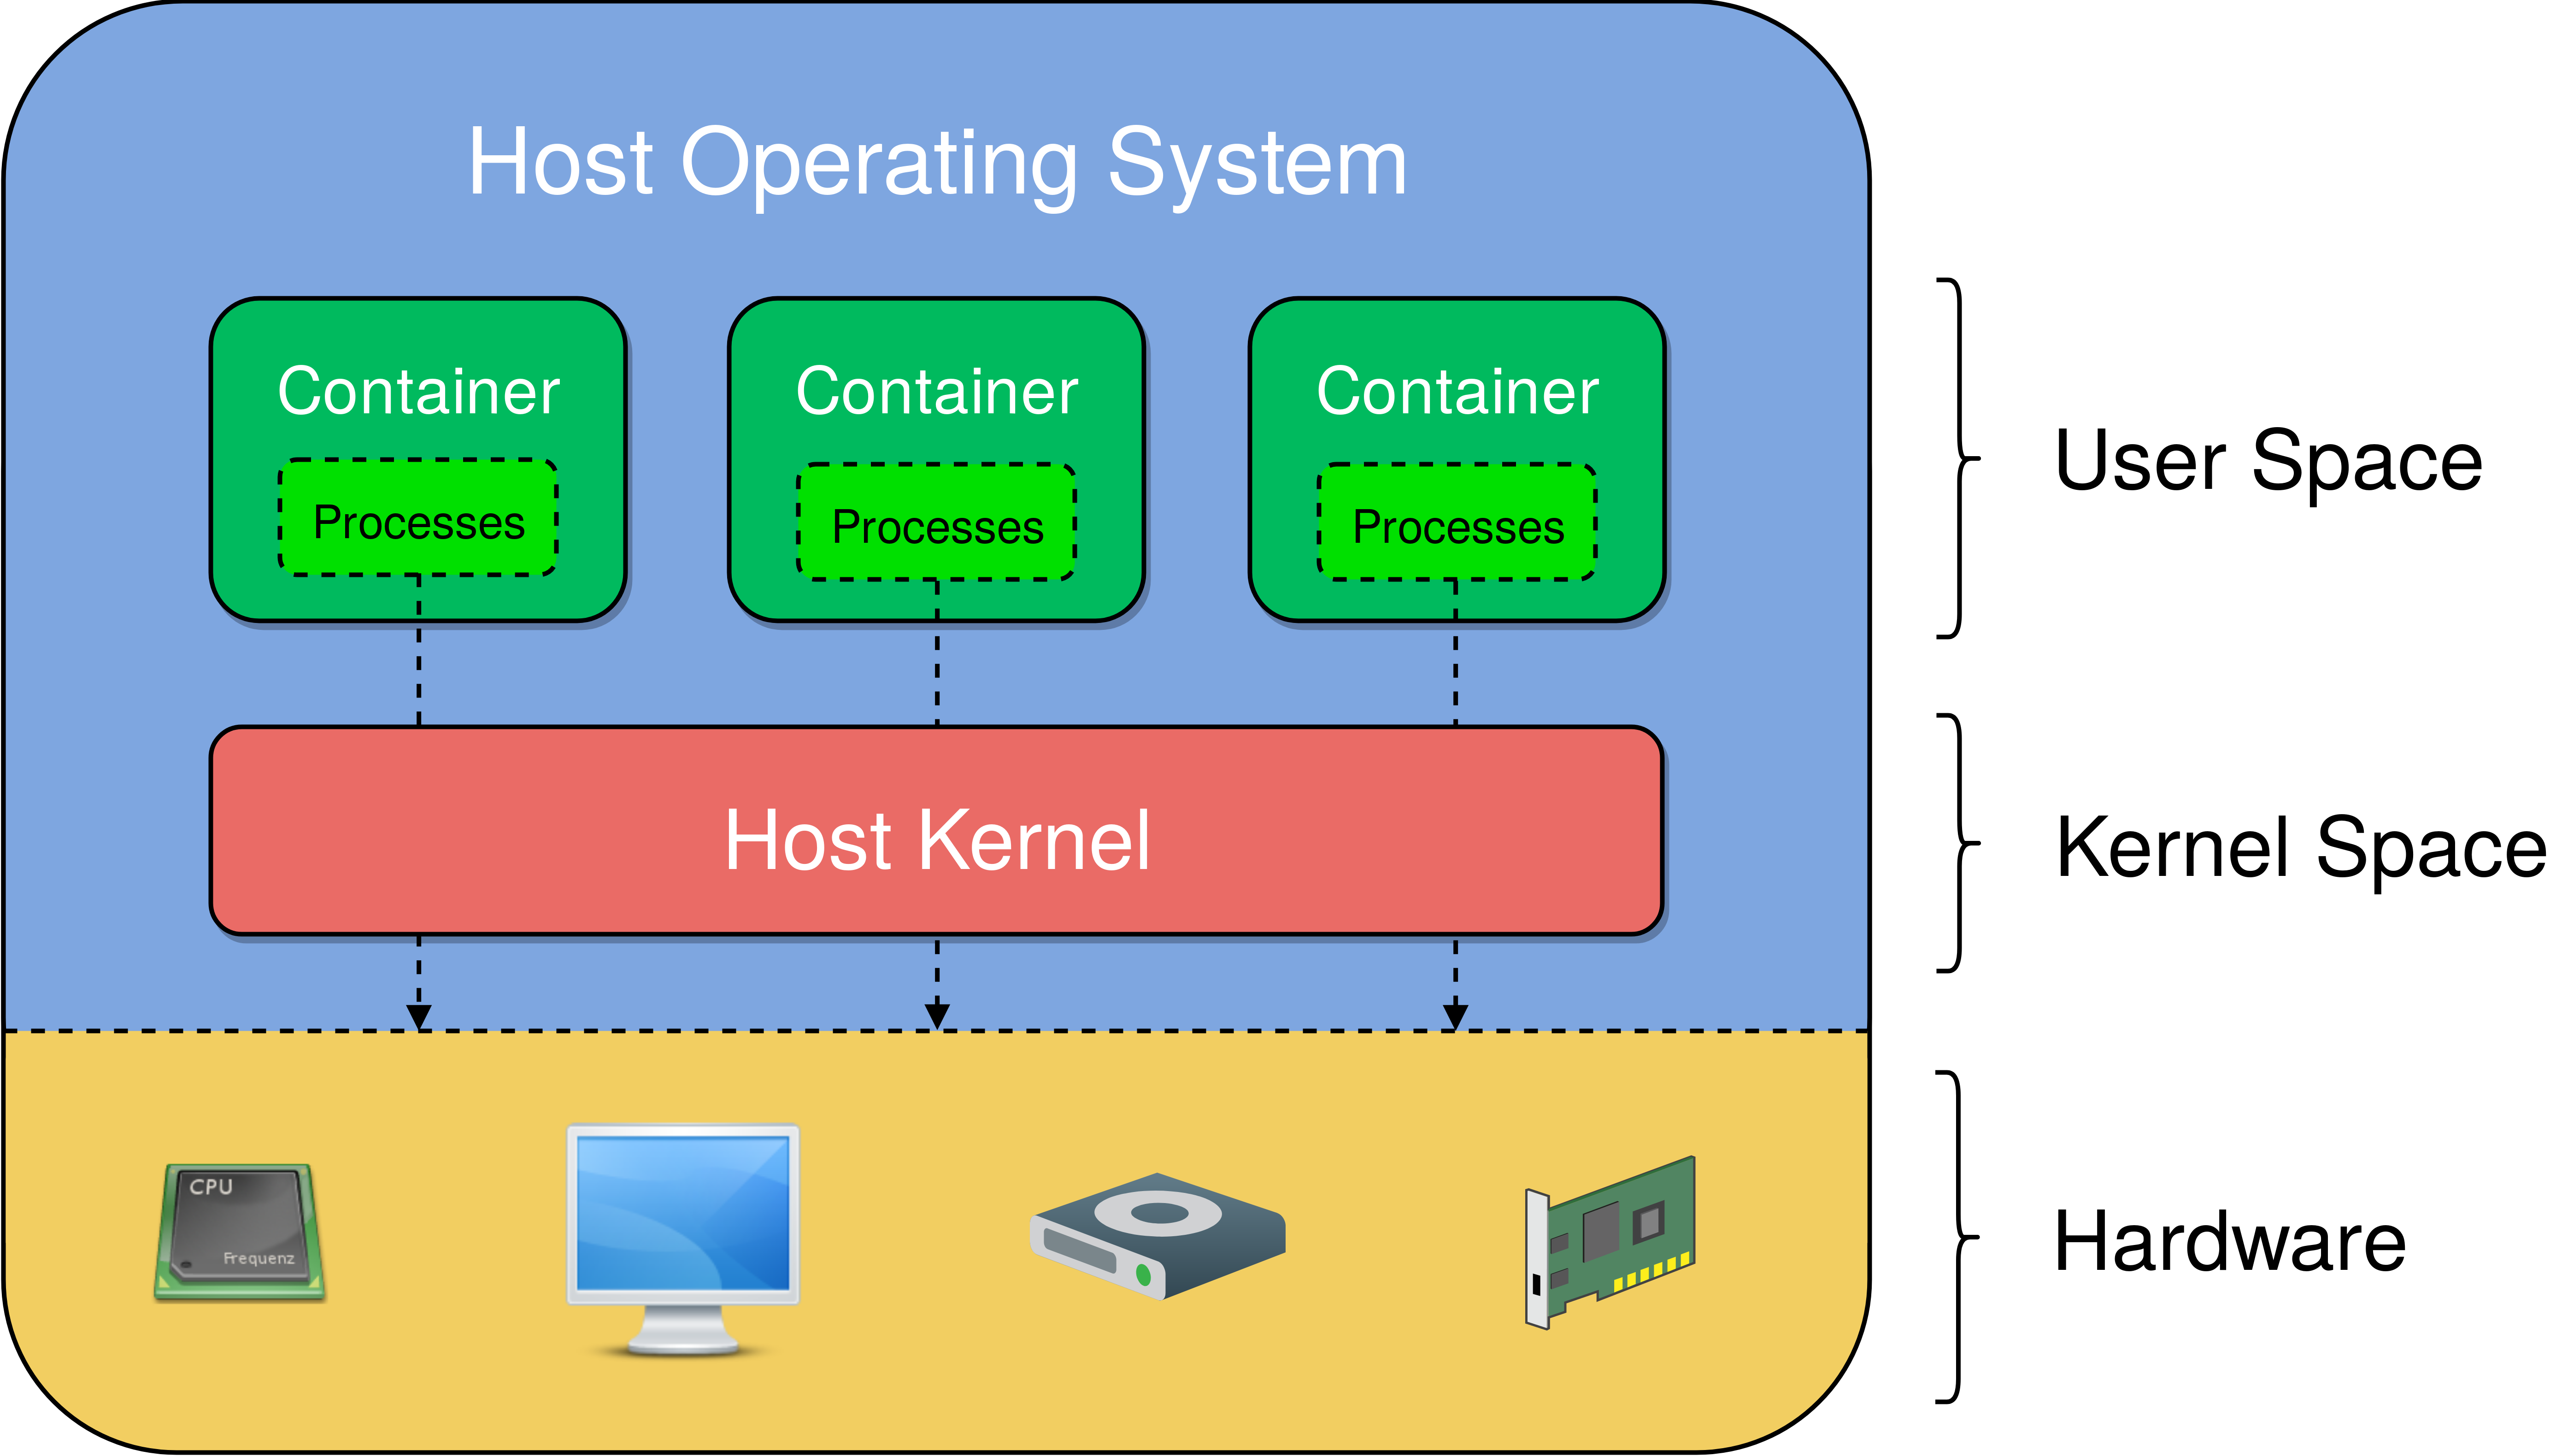
\includegraphics[width=0.65\textwidth]{../figures/user_kernel_hardware.png}
\caption{Containers live in user space. Par défaut, ils sont mis en bac à sable à partir de l'OS hôte et des conteneurs frères et sœurs, mais contrairement aux VM, ils partagent un noyau commun entre eux et avec l'OS hôte. Tous les appels système sont passés par le noyau hôte.}
\label{fig:user_kernel_hardware}
\end{figure}

Les conteneurs Docker sont des environnements d'exécution en bac à sable qui sont portables, reproductibles et dont la version est contrôlée. Chaque environnement contient toutes ses dépendances, mais reste isolé du système d'exploitation et du système de fichiers hôte. Docker fournit un mécanisme pour contrôler les ressources auxquelles chaque conteneur est autorisé à accéder, et fournit un espace de noms Linux séparé pour chaque conteneur, isolant efficacement le réseau, les utilisateurs et les montages du système de fichiers du système d'exploitation hôte. Contrairement aux machines virtuelles, les outils de virtualisation basés sur des conteneurs comme Docker sont adaptés aux SBC portables et peuvent fonctionner avec une surcharge proche de zéro par rapport aux processus Linux natifs. Un seul Raspberry Pi est capable d'exécuter simultanément des centaines de conteneurs sans dégradation notable des performances. Espace{-.08em}\footnote{\url{https://blog.docker.com/2015/09/update-raspberry-pi-dockercon-challenge/}}

Si la conteneurisation simplifie considérablement le processus de création et de déploiement des applications, elle introduit également une certaine complexité supplémentaire dans le cycle de vie du développement des logiciels. Docker, comme la plupart des plates-formes de conteneur, utilise un système de fichiers en couches. Cela permet à Docker de prendre une "image" existante et de la modifier en installant de nouvelles dépendances ou en modifiant ses fonctionnalités. Les images sont généralement construites comme une séquence de couches, chacune devant être mise à jour périodiquement. Il faut veiller, lors de la conception du pipeline de développement, à ce que ces mises à jour ne brisent pas silencieusement une couche suivante, comme nous le décrivons dans \autoref{sec:retrospective}.

\section{Introduction to Docker}\label{sec:docker-intro}

Supposons qu'il existe un programme connu pour fonctionner sur un ordinateur quelconque. Il serait bon de donner à un autre ordinateur -- n'importe quel ordinateur connecté à Internet -- une courte chaîne de caractères ASCII, d'appuyer sur les touches \keys{\return}, et de revenir pour voir ce même programme s'exécuter. Peu importe où le programme a été construit ou quel logiciel était en cours d'exécution à ce moment-là. Cela peut sembler trivial, mais c'est un problème monumental de génie logiciel. Divers gestionnaires de paquets ont tenté de résoudre ce problème, mais même lorsqu'ils fonctionnent comme prévu, ils ne prennent en charge que les binaires compilés en natif sur les systèmes d'exploitation ayant le même gestionnaire de paquets.

Docker\footnote{Le tutoriel suivant utilise Docker, mais le flux de travail décrit est similaire à celui de la plupart des plateformes de conteneurs.} est un outil de calcul portable et reproductible. Avec Docker, les utilisateurs peuvent exécuter n'importe quel programme Linux sur presque tous les appareils informatiques en réseau de la planète, quel que soit le système d'exploitation ou l'architecture matérielle sous-jacents. Toutes les étapes de préparation, d'installation et de configuration de l'environnement peuvent être automatisées du début à la fin. Selon la largeur de bande disponible sur le réseau, cela peut prendre un certain temps, mais les utilisateurs n'auront jamais besoin d'intervenir dans le processus d'installation.

Pour installer Docker lui-même, exécutez la commande suivante sur un shell conforme à POSIX de n'importe quelle \href{https://docs.docker.com/install/#supported-platforms}{Plateforme supportée par Docker}:

\begin{pclisting}
    ~$ curl -sSL https://get.docker.com/ | sh
\end{pclisting}
%
Un Docker \textit{image} est essentiellement un instantané du système de fichiers -- un fichier unique qui contient tout ce qui est nécessaire pour faire fonctionner un certain conteneur du Docker. Les images des Dockers sont hébergées dans des \textit{registres}, similaires aux dépôts Git ou aux serveurs VCS. La commande suivante permet d'extraire une image Docker, par exemple \inline{daphne/duck} du dépôt par défaut \hyperref[subsec:docker_hub]{Docker Hub}:

\begin{pclisting}
    ~$ docker pull (*@\hl{daphne/duck}@*)
\end{pclisting}
%
Chaque image du Docker a un identifiant, un nom et une étiquette:

\begin{pclisting}
~$ docker images
REPOSITORY      TAG        IMAGE ID         CREATED       SIZE
(*@\hl{daphne/duck}@*)     latest     ea2f90g8de9e     1 day ago     869MB
\end{pclisting}
%
Pour lancer un conteneur Docker, utilisez la commande suivante:

\begin{pclisting}
~$ docker run daphne/duck
\end{pclisting}
%
La commande suivante permet de vérifier que le conteneur est bien en cours d'exécution:

\begin{pclisting}
~$ docker ps
CONTAINER ID     IMAGE           ...     NAMES
52994ef22481     daphne/duck     ...     (*@\hl{happy\_hamster}@*)
\end{pclisting}
%
Notez que l'image de Daphné possède un identifiant alphanumérique du conteneur, \inline{52994ef22481}, une image de base, \inline{daphne/duck}, et un nom mémorable, \inline{happy\_hamster}. Ce nom est un alias pour l'ID du conteneur, qui peut être utilisé de manière interchangeable pour faire référence au conteneur.

Les images de docker peuvent être créées de deux manières différentes. Tout d'abord, dans \autoref{subsec:creating-an-image-snapshot}, nous verrons comment créer une image Docker en prenant un instantané d'un conteneur en cours d'exécution, puis dans \autoref{subsec:writing-an-image-recipe}, comment créer un nouveau conteneur Docker en utilisant un type de recette spécial, appelé \href{https://docs.docker.com/engine/reference/builder/}{\inline{Dockerfile}}.

\subsection{Creating an image snapshot}\label{subsec:creating-an-image-snapshot}}, comment créer un nouveau conteneur Docker en utilisant une recette spéciale, appelée \href{}{\inline{Dockerfile}}.

Lorsqu'un conteneur du Docker écrit sur son propre système de fichiers, ces modifications ne sont pas persistantes, sauf si elles sont appliquées à une nouvelle image. Par exemple, démarrez un conteneur avec un shell interactif:

\begin{pclisting}
~$ docker run -it daphne/duck /bin/bash
root@(*@\hl{295fd7879184}@*):/#
\end{pclisting}
%
Notez l'ID du conteneur : \inline{295fd7879184}. Si on écrit sur le disque et qu'on laisse le conteneur,

\begin{pclisting}
root@295fd7879184:/# touch (*@\hl{new\_file}@*) && ls -l
total 0
-rw-r--r-- 1 root root 0 May 21 20:52 (*@\hl{new\_file}@*)
root@295fd7879184:/# exit
\end{pclisting}
%
\inline{new\_file} ne sera pas persisté. Si nous relançons la même commande:

\begin{pclisting}
~$ docker run -it daphne/duck /bin/bash
root@18f13bb4571a:/# ls
root@18f13bb4571a:/# touch new_file1 && ls -l
total 0
-rw-r--r-- 1 root root 0 May 21 21:32 new_file1
\end{pclisting}
%
Il semble que le "nouveau fichier" ait disparu ! Remarquez que l'ID du conteneur (\inline{18f13bb4571a}) est maintenant différent. C'est parce que la commande \inline{docker run daphne/duck} a créé un nouveau conteneur à partir de l'image de base \inline{daphne/duck}, plutôt que de redémarrer le conteneur précédent. Pour voir tous les conteneurs sur un hôte Docker, exécutez la commande suivante:

\begin{pclisting}
~$ docker container ls -a
CONTAINER ID      IMAGE            STATUS             NAMES
295fd7879184      daphne/duck      Exited (130)       merry_manatee
18f13bb4571a      daphne/duck      Up 5 minutes       shady_giraffe
52994ef22481      daphne/duck      Up 10 minutes      happy_hamster
\end{pclisting}
%
Il semble que \inline{295fd7879184} alias \inline{merry\_manatee} ait survécu, mais il ne fonctionne plus. Chaque fois que le processus principal d'un conteneur (rappelons que nous avons exécuté \inline{merry\_manatee} avec \inline{/bin/bash}) se termine, le conteneur s'arrête, mais il ne cesse pas d'exister. En fait, nous pouvons reprendre le conteneur arrêté là où il s'est arrêté:
%
\begin{pclisting}
~$ docker start -a merry_manatee
root@295fd7879184:/# ls -l
total 0
-rw-r--r-- 1 root root 0 May 21 20:52 new_file
\end{pclisting}
%
Rien n'a été perdu ! Pour le vérifier, nous pouvons vérifier quels autres conteneurs sont en cours d'utilisation:

\begin{pclisting}
~$ docker ps
CONTAINER ID       IMAGE             ...       NAMES
295fd7879184       daphne/duck       ...       merry_manatee
18f13bb4571a       daphne/duck       ...       shady_giraffe
52994ef22481       daphne/duck       ...       happy_hamster
\end{pclisting}
%
Supposons maintenant que nous voulions partager le conteneur \inline{shady\_giraffe} avec quelqu'un d'autre. Pour ce faire, nous devons d'abord prendre un instantané du conteneur en cours d'utilisation, ou le placer dans une nouvelle image avec un nom et une balise. Cela créera un point de contrôle que nous pourrons restaurer ultérieurement:

\begin{pclisting}
~$ docker commit -m "forking daphne/duck" (*@\hl{shady\_giraffe}@*) user/duck:v2
\end{pclisting}
%
Pour faire référence au conteneur, on peut utiliser soit \inline{18f13bb4571a} soit le nom désigné, c'est-à-dire \inline{shady\_giraffe}. Ce dépôt d'images sera appelé \inline{user/duck}, et possède un identifiant de version optionnel, \inline{:v2}, qui peut être poussé dans le registre \hyperref[subsec:docker_hub]{Docker Hub}:

\begin{pclisting}
~$ docker push (*@\hl{user/duck:v2}@*)
~$ docker images
REPOSITORY    TAG        IMAGE ID         CREATED          SIZE
daphne/duck   latest     ea2f90g8de9e     1 day ago        869MB
user/duck     v2         d78be5cf073e     2 seconds ago    869MB
~$ docker pull user/duck:v2
~$ docker run user/duck:v2 ls -l
total 0
-rw-r--r-- 1 root root 0 May 21 21:32 new_file1
\end{pclisting}
%
C'est un moyen pratique de partager une image avec des collègues et des collaborateurs. Toute personne ayant accès au dépôt peut retirer cette image et continuer là où nous nous sommes arrêtés, ou créer une autre image basée sur le dessus.

\subsection{Writing an image recipe}\label{subsec:writing-an-image-recipe}

La deuxième façon de créer une image Docker est d'écrire une recette, appelée \inline{Dockerfile}. Un \inline{Dockerfile} est un fichier texte qui spécifie les commandes requises pour créer une image du Docker, généralement en modifiant une image de conteneur existante à l'aide d'une interface de script. Ils comportent également des \href{https://docs.docker.com/engine/reference/builder/}{mots-clés} spéciaux (qui sont traditionnellement \inline{CAPITALIZED}), comme \href{https://docs.docker.com/engine/reference/builder/#from}{\inline{FROM}}, \href{https://docs.docker.com/engine/reference/builder/#from}{\inline{RUN}}, \href{https://docs.docker.com/engine/reference/builder/#entrypoint}{\inline{ENTRYPOINT}} et ainsi de suite. Par exemple, créez un fichier appelé \inline{Dockerfile}} avec le contenu suivant:

\begin{dockerlisting}
FROM daphne/duck      # Defines the base image
RUN touch new_file1   # new_file1 will be part of our snapshot
CMD ls -l             # Default command run when container is started
\end{dockerlisting}
%
Maintenant, pour construire l'image, nous pouvons simplement courir:

\begin{pclisting}
~$ docker build -t user/duck:v3 (*@\hl{.}@*)
\end{pclisting}
%
Le \inline{.} indique le répertoire courant, qui doit être le même que celui contenant notre \inline{Dockerfile}. Cette commande devrait produire quelque chose comme la sortie suivante:

\begin{pclisting}
Sending build context to Docker daemon  2.048kB
Step 1/3 : FROM daphne/duck
--- ea2f90g8de9e
Step 2/3 : RUN touch new_file1
--- e3b75gt9zyc4
Step 3/3 : CMD ls -l
--- Running in 14f834yud59
Removing intermediate container 14f834yud59
--- 05a3bd381fc2
Successfully built 05a3bd381fc2
Successfully tagged user/duck:v3
\end{pclisting}
%
La commande, \inline{docker images} devrait afficher une image appelée \inline{user/duck:v3}:

\begin{pclisting}
~$ docker images
REPOSITORY    TAG        IMAGE ID         CREATED          SIZE
daphne/duck   latest     ea2f90g8de9e     1 day ago        869MB
user/duck     v2         d78be5cf073e     5 minutes ago    869MB
user/duck     v3         05a3bd381fc2     2 seconds ago    869MB
\end{pclisting}
%
Cette procédure est identique à la technique d'instantané réalisée dans \autoref{subsec:creating-an-image-snapshot}, mais le résultat est plus propre. Plutôt que de conserver une image de 869 Mo, on peut se contenter de stocker le fichier texte de 4 Ko. Pour exécuter l'image résultante, nous pouvons simplement utiliser la même commande qu'auparavant:

\begin{pclisting}
~$ docker run -it (*@\hl{user/duck:v3}@*)
total 0
-rw-r--r-- 1 root root 0 May 21 21:35 new_file1
\end{pclisting}
%
Notez que dès que nous lançons le conteneur, Docker exécute la commande \inline{ls -l} comme spécifié par le \inline{Dockerfile}, révélant que \inline{new\_file1} a bien été stocké dans l'image. Cependant, cette commande par défaut peut être remplacée par une commande personnalisée:

\begin{pclisting}
~$ docker run -it user/duck:v3 (*@\hl{[custom command]}@*)
\end{pclisting}
%
\subsection{Layer caching}

\href{https://docs.docker.com/storage/storagedriver/#images-and-layers}{Layers} sont un concept important à comprendre quand on travaille avec Docker. Une façon de penser à une couche est comme un commit Git -- un ensemble de modifications à une image ou une couche précédente, identifiée de façon unique par un code de hachage. Dans un \inline{Dockerfile}, les calques commencent par un \href{https://docs.docker.com/engine/reference/builder/#from}{mot-clé}.

\begin{dockerlisting}
FROM daphne/duck
RUN touch new_file1                            # Defines a new layer
RUN mkdir config && mv new_file1 config        # Layers can chain commands
RUN apt-get update && apt-get install -y wget  # Install a dependency
RUN wget https://get.your.app/install.sh       # Download a script
RUN chmod +x install.sh && ./install.sh        # Run the script
\end{dockerlisting}
%
Pour construire cette image, nous pouvons exécuter la commande suivante:

\begin{pclisting}
~$ docker build -t user/duck:v4 .
Sending build context to Docker daemon  2.048kB
Step 1/6 : FROM daphne/duck
---> cd6d8154f1e1
...
Removing intermediate container 8fb56ef38bc8
---> 3358ca1b8649
Step 5/6 : RUN wget https://get.your.app/install.sh
---> Running in e8284ff4ec8b
...
2018-10-30 06:47:57 (89.9 MB/s) - 'install.sh' saved [13847/13847]
Removing intermediate container e8284ff4ec8b
---> 24a22dc2900a
Step 6/6 : RUN chmod +x install.sh && ./install.sh
---> Running in 9526651fa492
# Executing install script, commit: 36b78b2
...
Removing intermediate container 9526651fa492
---> a8be23fea573
Successfully built a8be23fea573
Successfully tagged user/duck:v4
\end{pclisting}
%
Les couches sont mises en cache de manière pratique par le \href{https://docs.docker.com/engine/reference/commandline/dockerd/}{Docker daemon}. Si nous devons exécuter deux fois la même commande, Docker utilisera le cache au lieu de reconstruire l'image entière:

\begin{pclisting}
Sending build context to Docker daemon  2.048kB
Step 1/6 : FROM daphne/duck
---> cd6d8154f1e1
Step 2/6 : RUN touch new_file1
---> (*@\hl{Using cache}@*)
---> 0473154b2004
...
Step 6/6 : RUN chmod +x index.html && ./index.html
---> (*@\hl{Using cache}@*)
---> a8be23fea573
Successfully built a8be23fea573
Successfully tagged user/duck:v4
\end{pclisting}
%
Si nous devons apporter une modification au \inline{Dockerfile}, Docker ne reconstruira l'image qu'à partir de la première étape modifiée. Supposons que nous ajoutions une nouvelle commande \inline{RUN} à la fin de notre \inline{Dockerfile} et que nous déclenchions une reconstruction de la même manière:

\begin{pclisting}
~$ echo 'RUN echo "(*@\hl{Change here!}@*)"' >> Dockerfile
~$ docker build -t user/duck:v4 .
Sending build context to Docker daemon  2.048kB
...
Step 6/7 : RUN chmod +x index.html && ./index.html
---> Using cache
---> a8be23fea573
Step 7/7 : RUN echo "Change here!"
---> Running in 80fc5c402304
(*@\hl{Change here!}@*)
Removing intermediate container 80fc5c402304
---> c1ec64cef9c6
Successfully built c1ec64cef9c6
Successfully tagged user/duck:v4
\end{pclisting}
%
Si Docker devait relancer l'ensemble du [fichier] en ligne de haut en bas à chaque reconstruction, cela serait lent et peu pratique. Au lieu de cela, Docker met en cache les étapes non modifiées par défaut, et ne refait que le minimum d'étapes nécessaires à la reconstruction. Cela peut parfois donner des résultats inattendus, surtout lorsque la cache est périmée. Pour ignorer le cache et forcer une reconstruction propre, utilisez l'indicateur \inline{-{}-no-cache} lors de la construction d'un \inline{Dockerfile}.

Que prend en compte Docker pour décider d'utiliser le cache? Tout d'abord, le \inline{Dockerfile} lui-même - lorsqu'une étape d'un \inline{Dockerfile} change, elle et toutes les étapes suivantes devront être relancées lors de la compilation. Docker vérifie également le \href{https://docs.docker.com/engine/reference/commandline/build/#extended-description}{contexte de construction} pour les changements. Lorsque \inline{docker build -t TAG .} est écrit, le \inline{.} indique le contexte de construction, ou le chemin où la construction doit avoir lieu. Souvent, ce chemin contient des artefacts de compilation. Par exemple:

\begin{dockerlisting}
FROM daphne/duck
COPY duck.txt .
RUN cat duck.txt
\end{dockerlisting}
%
Maintenant, si nous ajoutons un message dans \inline{duck.txt} et reconstruisons notre image, le fichier sera copié dans l'image du Docker, et son contenu sera imprimé:

\begin{pclisting}
~$ echo "(*@\hl{Make way!}@*)" > duck.txt && docker build -t user/duck:v5 .
Sending build context to Docker daemon  3.072kB
Step 1/3 : FROM daphne/duck
---> cd6d8154f1e1
Step 2/3 : COPY duck.txt .
---> e0e03d9e1791
Step 3/3 : RUN cat duck.txt
---> Running in 590c5420ce29
(*@\hl{Make way!}@*)
Removing intermediate container 590c5420ce29
---> 1633e3e10bef
Successfully built 1633e3e10bef
Successfully tagged user/duck:v5
\end{pclisting}
%
Tant que les trois premières lignes du \inline{Dockerfile} et du \inline{duck.txt} ne sont pas modifiées, ces couches seront mises en cache et Docker ne les reconstruira pas. Si le contenu du fichier \inline{duck.txt} est modifié par la suite, cela déclenchera une reconstruction. Par exemple, si nous ajoutons au fichier et le reconstruisons, seules les deux dernières étapes devront être exécutées:

\begin{pclisting}
~$ echo "(*@\hl{Thank you. Have a nice day!}@*)" >> duck.txt
~$ docker build -t user/duck:v5 .
Sending build context to Docker daemon  3.072kB
Step 1/3 : FROM ubuntu
---> cd6d8154f1e1
Step 2/3 : COPY duck.txt .
---> f219efc150a5
Step 3/3 : RUN cat duck.txt
---> Running in 7c6f5f8b73e9
(*@\hl{Make way!}@*)
(*@\hl{Thank you. Have a nice day!}@*)
Removing intermediate container 7c6f5f8b73e9
---> e8a1db712aee
Successfully built e8a1db712aee
Successfully tagged user/duck:v5
\end{pclisting}
%
Une erreur courante lors de l'écriture de \inline{Dockerfile}s consiste à \inline{COPY} plus de fichiers que ce qui est strictement nécessaire pour effectuer l'étape de construction suivante. Par exemple, si \inline{COPY . .} est écrit au début du \inline{Dockerfile}, chaque fois qu'un fichier est modifié dans le contexte de la compilation, cela déclenchera une reconstruction de toutes les étapes de compilation suivantes. Afin de maximiser la réutilisation du cache et de réduire au minimum le temps de reconstruction, les utilisateurs doivent être aussi prudents que possible et ne \inline{COPY} que le minimum de fichiers nécessaires pour accomplir l'étape de construction suivante.

% Comme le \inline{.gitignore} de Git, Docker a également un fichier \inline{.dockerignore}. Si nous ajoutons une ligne au fichier \inline{.dockerignore}, alors tous les chemins correspondant à cette ligne dans le contexte de compilation seront ignorés. Docker accepte également d'autres motifs comme les expressions régulières et la négation.~\footnote{Further details : \url{https://docs.docker.com/engine/reference/builder/#dockerignore-file}}

\subsection{Volume sharing}\label{subsec:volume_sharing}

Il existe une deuxième méthode pour déposer les données dans un conteneur, qui ne nécessite pas de les intégrer dans l'image mère au moment de la compilation. Cette méthode est plus appropriée pour les données qui sont nécessaires au moment de l'exécution, mais non essentielles pour la construction. Elle prend la forme suivante:

\begin{pclisting}
~$ docker run user/duck:v6 (*@\hl{-v HOST\_PATH:TARGET\_PATH}@*)
\end{pclisting}
%
Supposons que nous ayons un \inline{Dockerfile} qui fournit une instruction \inline{CMD} par défaut:

\begin{dockerlisting}
de daphne/duck
CMD /bin/bash -c "/launch.sh"
\end{dockerlisting}
%
Si nous construisions cette image et essayions de l'exécuter, le fichier \inline{/launch.sh} serait manquant:

\begin{pclisting}
~$ docker build -t user/duck:v6 && docker run user/duck:v6
bash: (*@\hl{/launch.sh}@*): No such file or directory
\end{pclisting}
%
Au lieu de cela, lorsque nous utilisons le conteneur, nous devons partager le fichier via le Docker CLI:

\begin{pclisting}
~$ echo -e '#!/bin/bash\necho Launching...' >> launch.sh && \
   chmod 775 launch.sh && \
   docker run user/duck:v6 (*@\hl{-v launch.sh:/launch.sh}@*)
Launching...
\end{pclisting}
%
De cette façon, le fichier local \inline{launch.sh} sera disponible pour être utilisé à l'intérieur du conteneur au chemin désigné, \inline{/launch.sh}.

\subsection{Multi-stage builds}

Le système de fichiers de Docker est additif, donc chaque couche ne fera qu'augmenter la taille de l'image finale. Pour cette raison, il est souvent nécessaire de mettre de l'ordre dans les fichiers inutiles après l'installation. Par exemple, lors de l'installation de dépendances sur des images basées sur Debian, il est courant de les exécuter:

\begin{dockerlisting}
RUN apt-get update && apt-get install ... && (*@\hl{rm -rf /var/lib/apt/lists/*}@*)
\end{dockerlisting}
%
Cela garantit que la liste des paquets n'est pas intégrée à l'image (Docker ne vérifie le calque qu'une fois chaque étape terminée). Les constructions peuvent souvent consommer plusieurs étapes, bien qu'elles ne produisent qu'un seul artefact. Au lieu d'enchaîner plusieurs commandes et de nettoyer les changements en une seule étape, les constructions à plusieurs étapes nous permettent de construire une série d'images à l'intérieur d'un \inline{Dockerfile}, et de copier les ressources de l'une à l'autre, en éliminant tous les artefacts de construction intermédiaires:

\begin{dockerlisting}
FROM user/duck:v3 as template1

FROM daphne/duck as template2
COPY --from=template1 new_file1 new_file2
FROM donald/duck as template3
COPY --from=template2 new_file2 (*@\hl{new\_file3}@*)
CMD ls -l
\end{dockerlisting}
%
Nous pouvons maintenant construire et faire fonctionner cette image comme suit:

\begin{pclisting}
~$ docker build . -t user/duck:v4
Sending build context to Docker daemon  2.048kB
Step 1/6 : FROM user/duck:v3 as template1
--- e3b75ef8ecc4
Step 2/6 : FROM daphne/duck as template2
--- ea2f90g8de9e
Step 3/6 : COPY --from=template1 new_file1 new_file2
---> 72b96668378e
Step 4/6 : FROM donald/duck:v3 as template3
---> e3b75ef8ecc4
Step 5/6 : COPY --from=template2 new_file2 (*@\hl{new\_file3}@*)
---> cb1b84277228
Step 6/6 : CMD ls
---> Running in cb1b84277228
Removing intermediate container cb1b84277228
---> c7dc5dd63e77
Successfully built c7dc5dd63e77
Successfully tagged user/duck:v4
~$ docker run -it user/duck:v4
total 0
-rw-r--r-- 1 root root 0 Jul  8 15:06 (*@\hl{new\_file3}@*)
\end{pclisting}
%
Une des applications des constructions en plusieurs étapes consiste à compiler une dépendance de projet à partir de son code source. En plus de tout le code source, le processus de compilation pourrait introduire des gigaoctets d'artefacts de construction et de dépendances transitives, juste pour construire un seul binaire. Les compilations multi-étapes nous permettent de construire le fichier, et de le copier sur une nouvelle couche, libérée des fichiers intermédiaires.

\section{ROS and Docker}\label{sec:ros-docker}

\begin{figure}[ht]
\centering
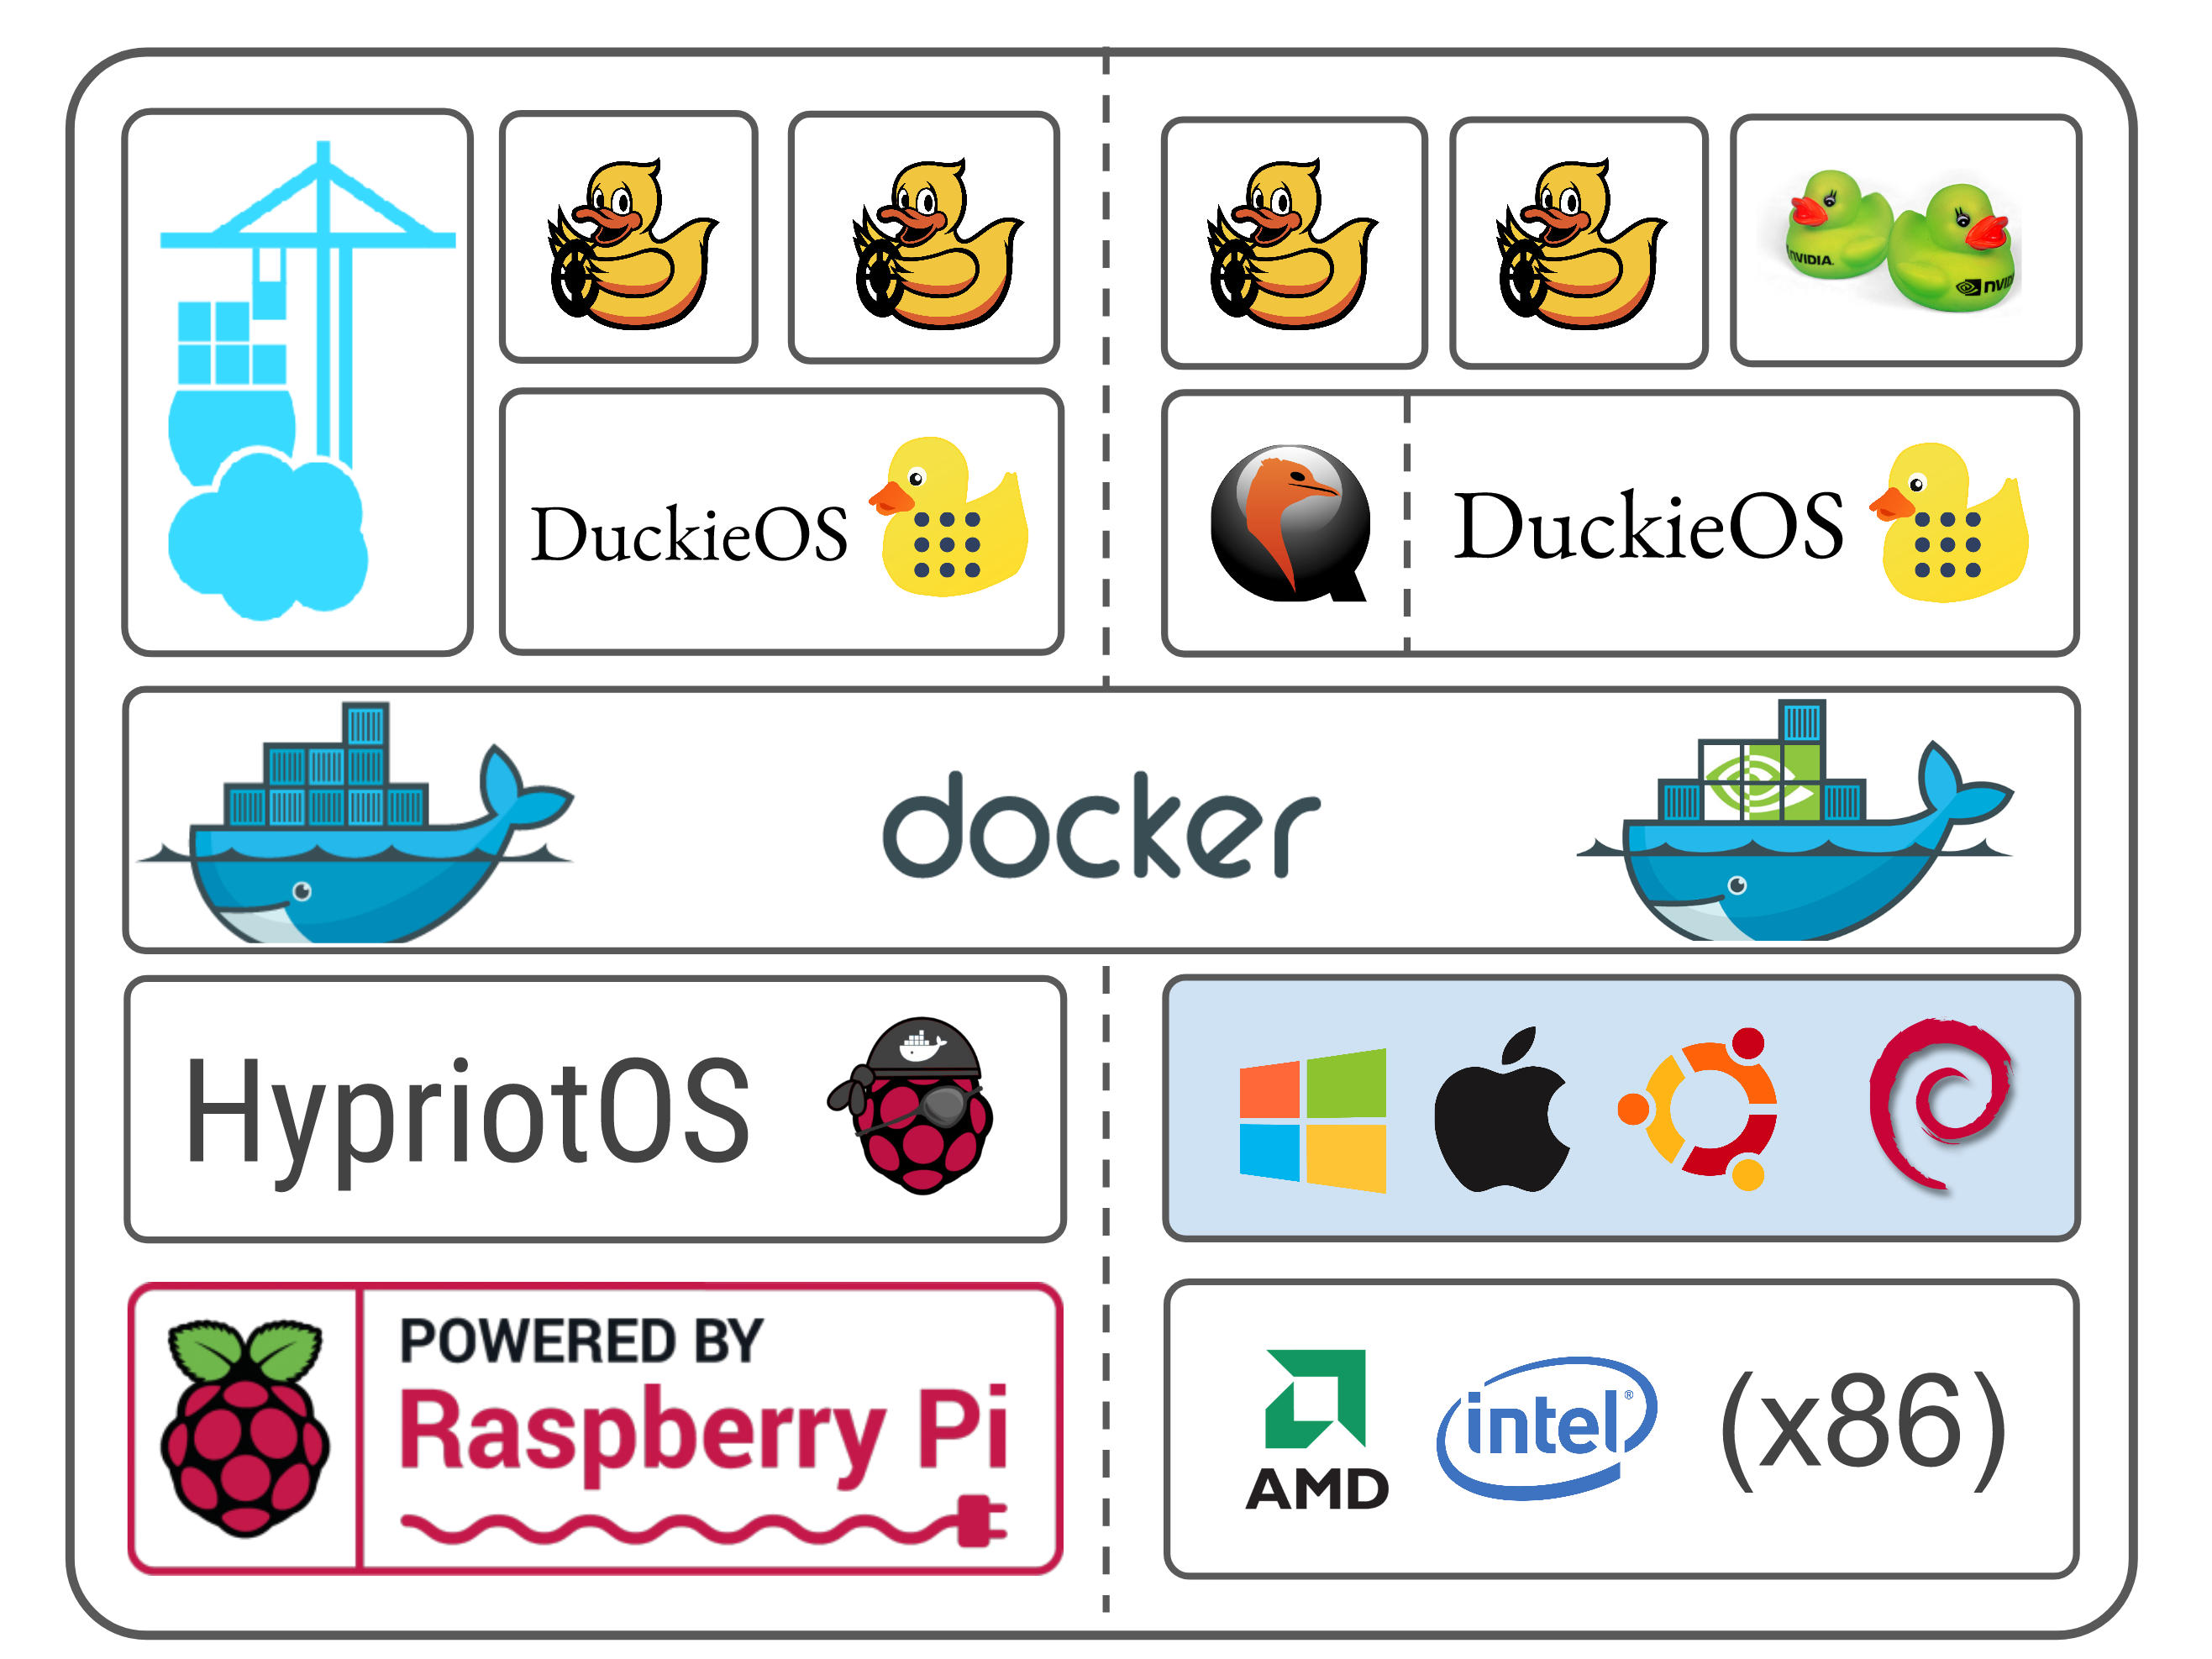
\includegraphics[width=0.48\textwidth]{../figures/docker_stack_1.png}
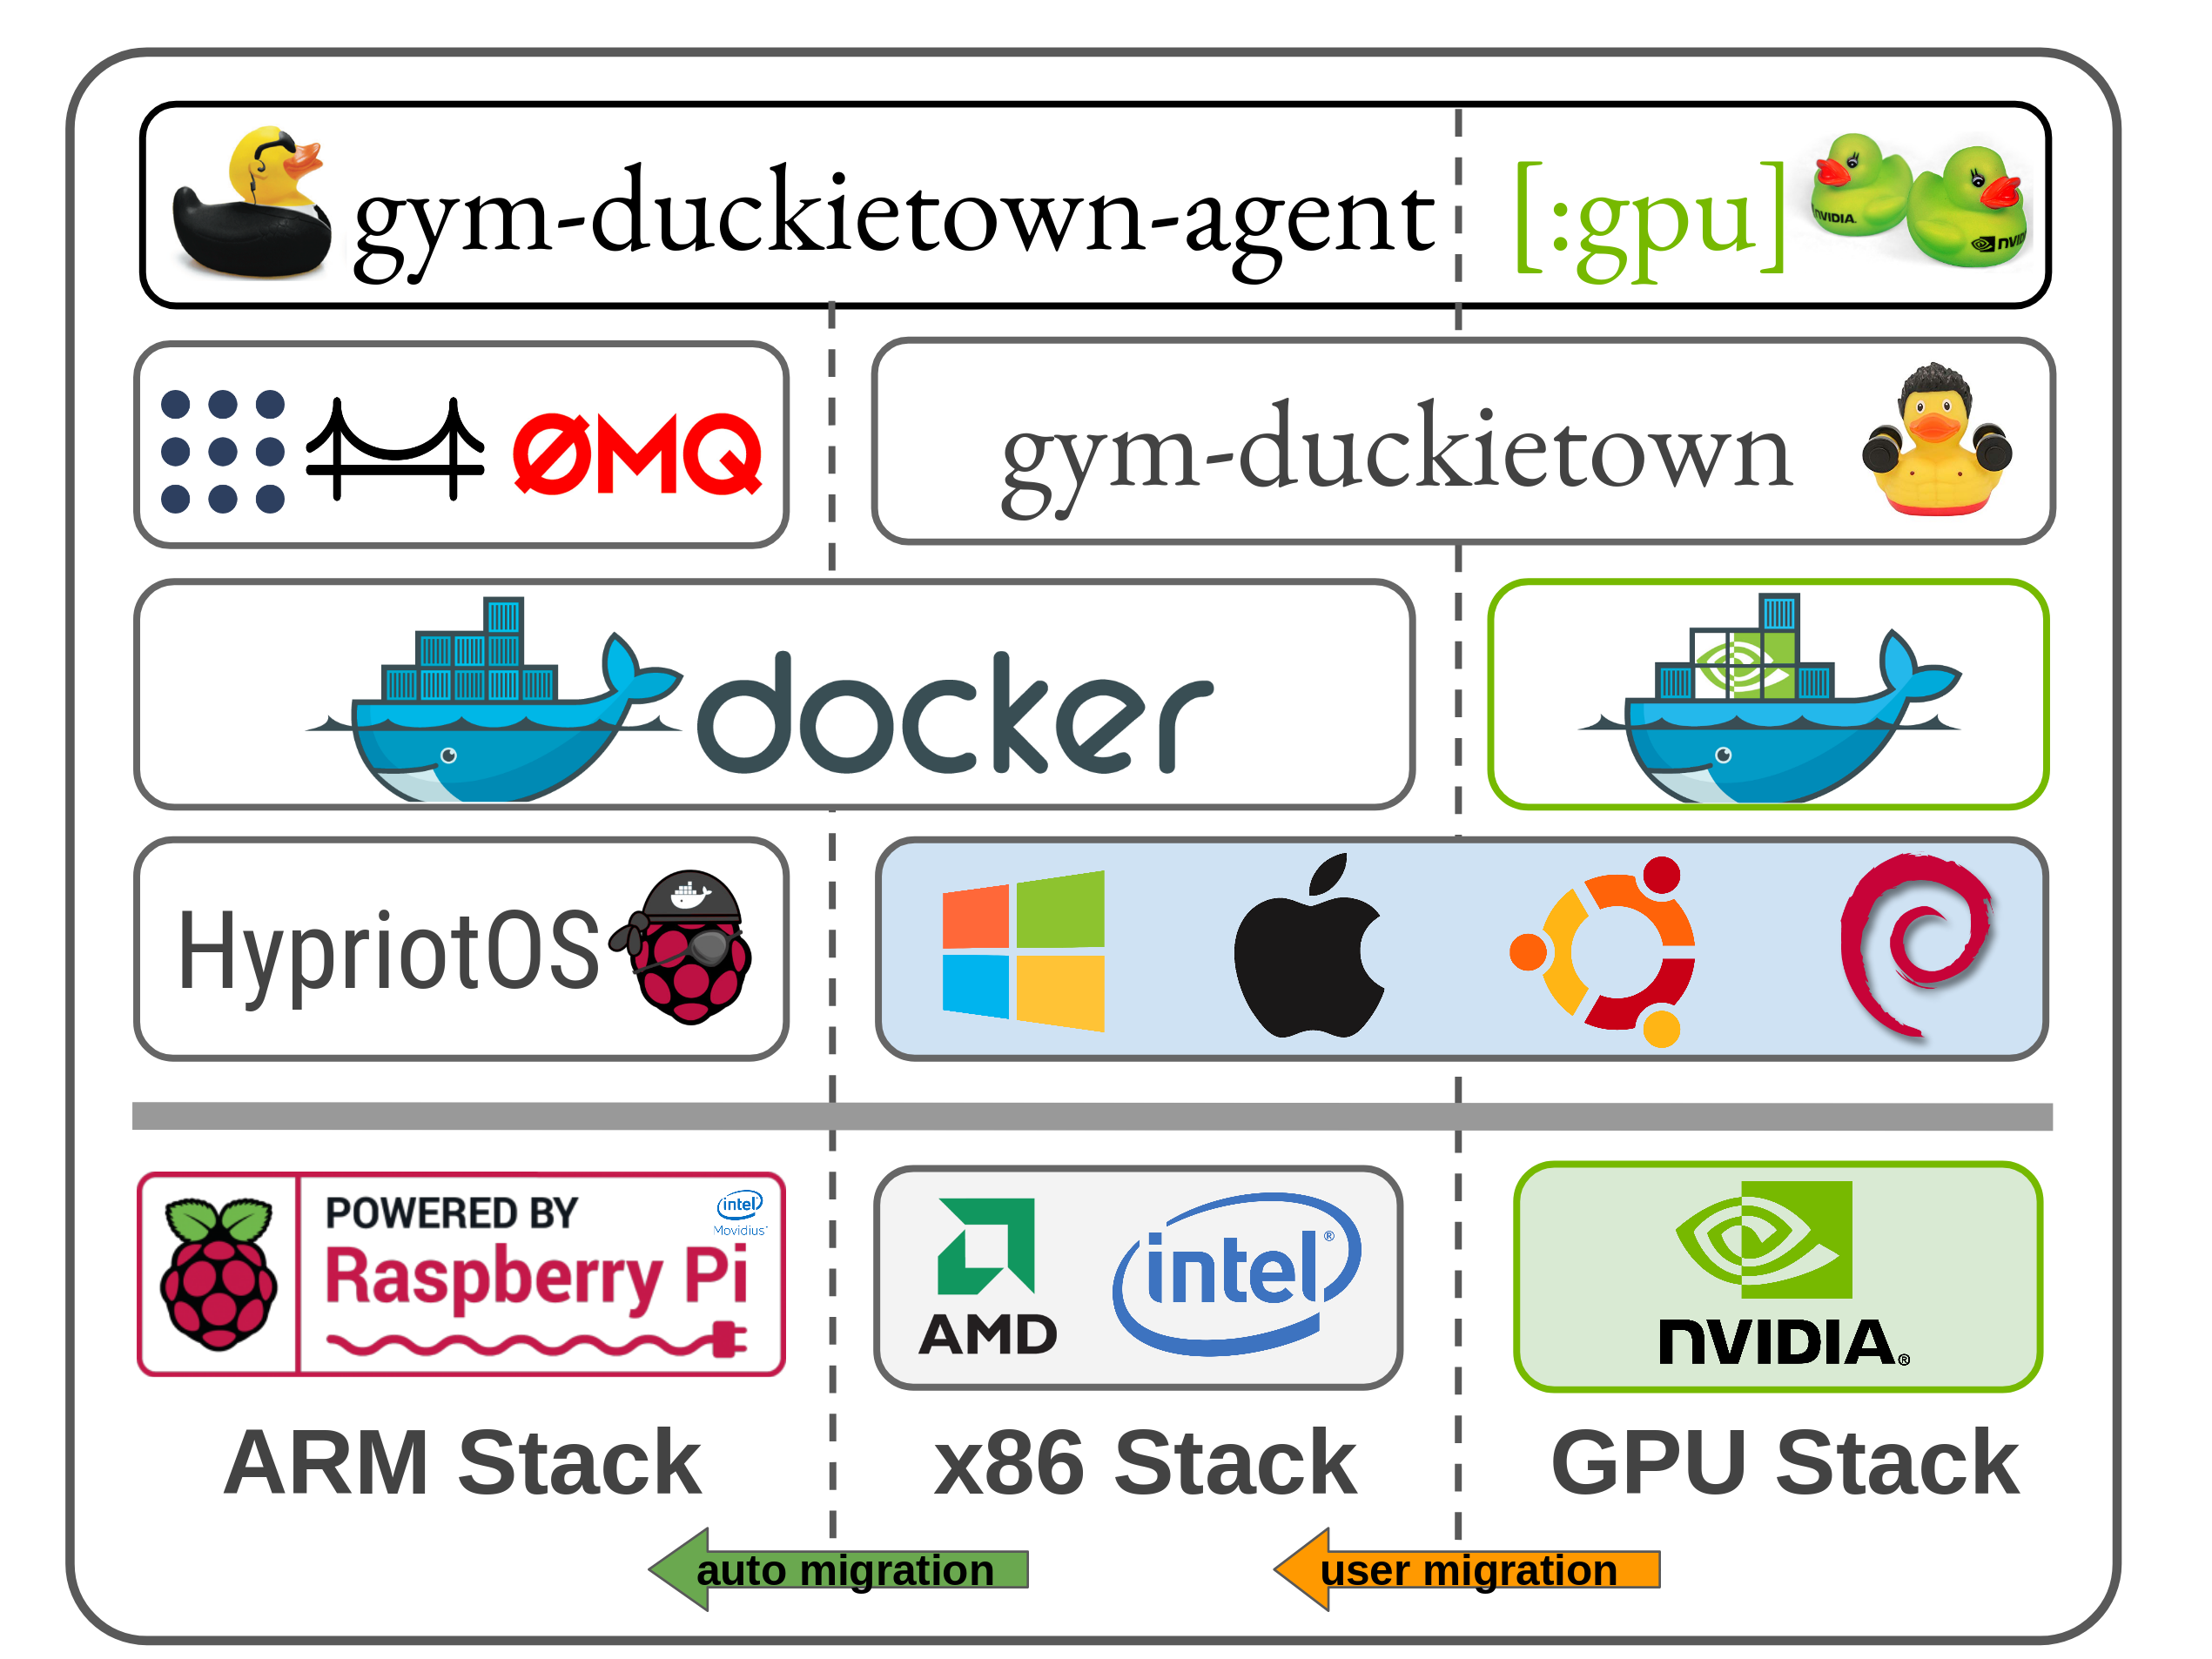
\includegraphics[width=0.48\textwidth]{../figures/docker_stack_2.png}
\caption{Infrastructure des conteneurs. \textbf{Gauche} : La pile ROS cible deux architectures primaires, x86 et ARM. Pour simplifier le processus de construction, nous construisons des artefacts ARM sur x86 en utilisant \href{https://www.qemu.org}{QEMU}~\citep{bellard2005qemu}. \textbf{Right} : Pile d'apprentissage de renforcement. Les artefacts de construction sont formés sur un GPU, et transférés sur le CPU pour évaluation. Les modèles d'apprentissage profond peuvent également être exécutés sur un dispositif ARM à l'aide d'un \href{https://software.intel.com/en-us/neural-compute-stick}{accélérateur}.}
\label{fig:docker}
\end{figure}

\citet{white2017ros-docker} a précédemment exploré les ROS Dockerizing, dont les travaux constituent la base des nôtres, qui étendent leur mise en œuvre à la plateforme Duckietown~\citep{paull2017duckietown}, un ensemble d'applications ROS plus spécifiques au matériel et au domaine.

La \href{https://www.duckietown.org}{platforme Duckietown} supporte deux architectures de jeu d'instructions primaires : x86 et ARM. Pour assurer la compatibilité d'exécution des paquets de Duckietown, nous effectuons une construction croisée en utilisant la virtualisation matérielle pour garantir que les artefacts de construction peuvent être exécutés sur l'une ou l'autre des architectures cibles. L'émulation en temps réel d'artefacts étrangers est également possible, en utilisant une technique similaire. Pour plus d'informations, cette technique est décrite plus en détail à l'URL suivante : \url{https://www.balena.io/blog/building-arm-containers-on-any-x86-machine-even-dockerhub/}.} Par souci de performance et de simplicité, nous n'utilisons l'émulation que lorsque cela est nécessaire (par exemple sur les appareils x86). Sur ARM-native, le système d'exploitation de base est \hyperref[subsec:hypriot]{HypriotOS}, une distribution Debian légère pour le Raspberry Pi et autres SBCs basés sur ARM, avec un support natif pour Docker. Pour les systèmes x86 et ARM, Docker est la plate-forme de conteneur sous-jacente sur laquelle toutes les applications utilisateur sont exécutées, à l'intérieur d'un conteneur. Comme ROS et Docker ont tous deux des interfaces de ligne de commande étendues, une interface unifiée, le \href{https://github.com/duckietown/duckietown-shell}{Duckietown Shell} (\inline{dts}), est fourni pour envelopper leur fonctionnalité et effectuer des tâches communes.

\section{Duckiebot development using Docker}

\noindent Le développement du logiciel pour la plate-forme Duckietown nécessite les objets physiques suivants:
%
\begin{enumerate}
\item Duckiebot (y compris appareil photo, roues et Raspberry Pi 3B+)\footnote{La liste complète des matériaux peut être trouvée à l'URL suivante : \url{https://get.duckietown.org/}}
\item Carte Micro SD (16GB+ recommandé)
\item Ordinateur personnel
\item Routeur Internet
\item Adaptateur de carte MicroSD
\end{enumerate}
%
En outre, nous supposons que les dépendances logicielles suivantes ont été installées sur (3):
%
\begin{enumerate}[label=(\alph*)]
\item \href{https://get.docker.com}{Docker CE}
\item POSIX-compliant shell
\item \inline{dts}, the Duckietown shell\footnote{May be obtained at the following URL : \url{https://github.com/duckietown/duckietown-shell}}
\item un navigateur Web (par exemple \href{https://www.google.com/chrome/}{Chrome} ou \href{https://mozilla.org/firefox/}{Firefox})
\item \inline{wget}/\inline{curl}
\end{enumerate}

\noindentent Le flux de travail suivant a été testé de manière approfondie sur des hôtes Linux fonctionnant sous Ubuntu 16.04 (et dans une moindre mesure, sous Mac OS X et VM). Aucune autre dépendance n'est supposée ou requise.

\subsection{Flashing a bootable disk}

L'une des premières étapes du Duckiebook exige des utilisateurs qu'ils installent manuellement un système d'exploitation personnalisé sur un support amorçable, un processus fastidieux et long. Le script d'installation suivant a été écrit pour automatiser ce processus, permettant aux utilisateurs de configurer plus facilement un environnement logiciel reproductible:

\begin{pclisting}
~$ bash -c "(*@\$@*)(wget -O- h.ndan.co)"
\end{pclisting}
%
Maintenant, avec le \href{https://github.com/duckietown/duckietown-shell}{Duckietown Shell}, la commande suivante est tout ce qu'il faut:
%
\begin{dtslisting}
dt> init_sd_card [--hostname "DUCKIEBOT_NAME"] [--wifi "username:password"]
\end{dtslisting}
%
Les utilisateurs doivent insérer une carte SD et suivre les instructions fournies. Une fois terminée, la carte est retirée et insérée dans la fente pour carte SD du Raspberry Pi. Au premier démarrage, il faut veiller à ce que l'appareil soit alimenté en continu pendant au moins dix minutes afin de permettre la fin de l'installation et d'éviter la corruption du système de fichiers.

\subsection{Web interface}

Pour accéder à l'interface web de DuckieOS, les utilisateurs peuvent visiter l'URL suivante dans n'importe quel navigateur web compatible JavaScript : \url{http://DUCKIEBOT_NAME:9000/}. Si le processus d'installation s'est achevé avec succès et que le réseau est correctement configuré, l'application web affichée dans~\autoref{fig:portainer_ui} devrait être accessible. Cette application permet aux utilisateurs non familiers avec le CLI de gérer les conteneurs Docker depuis leur navigateur préféré.

\begin{figure}
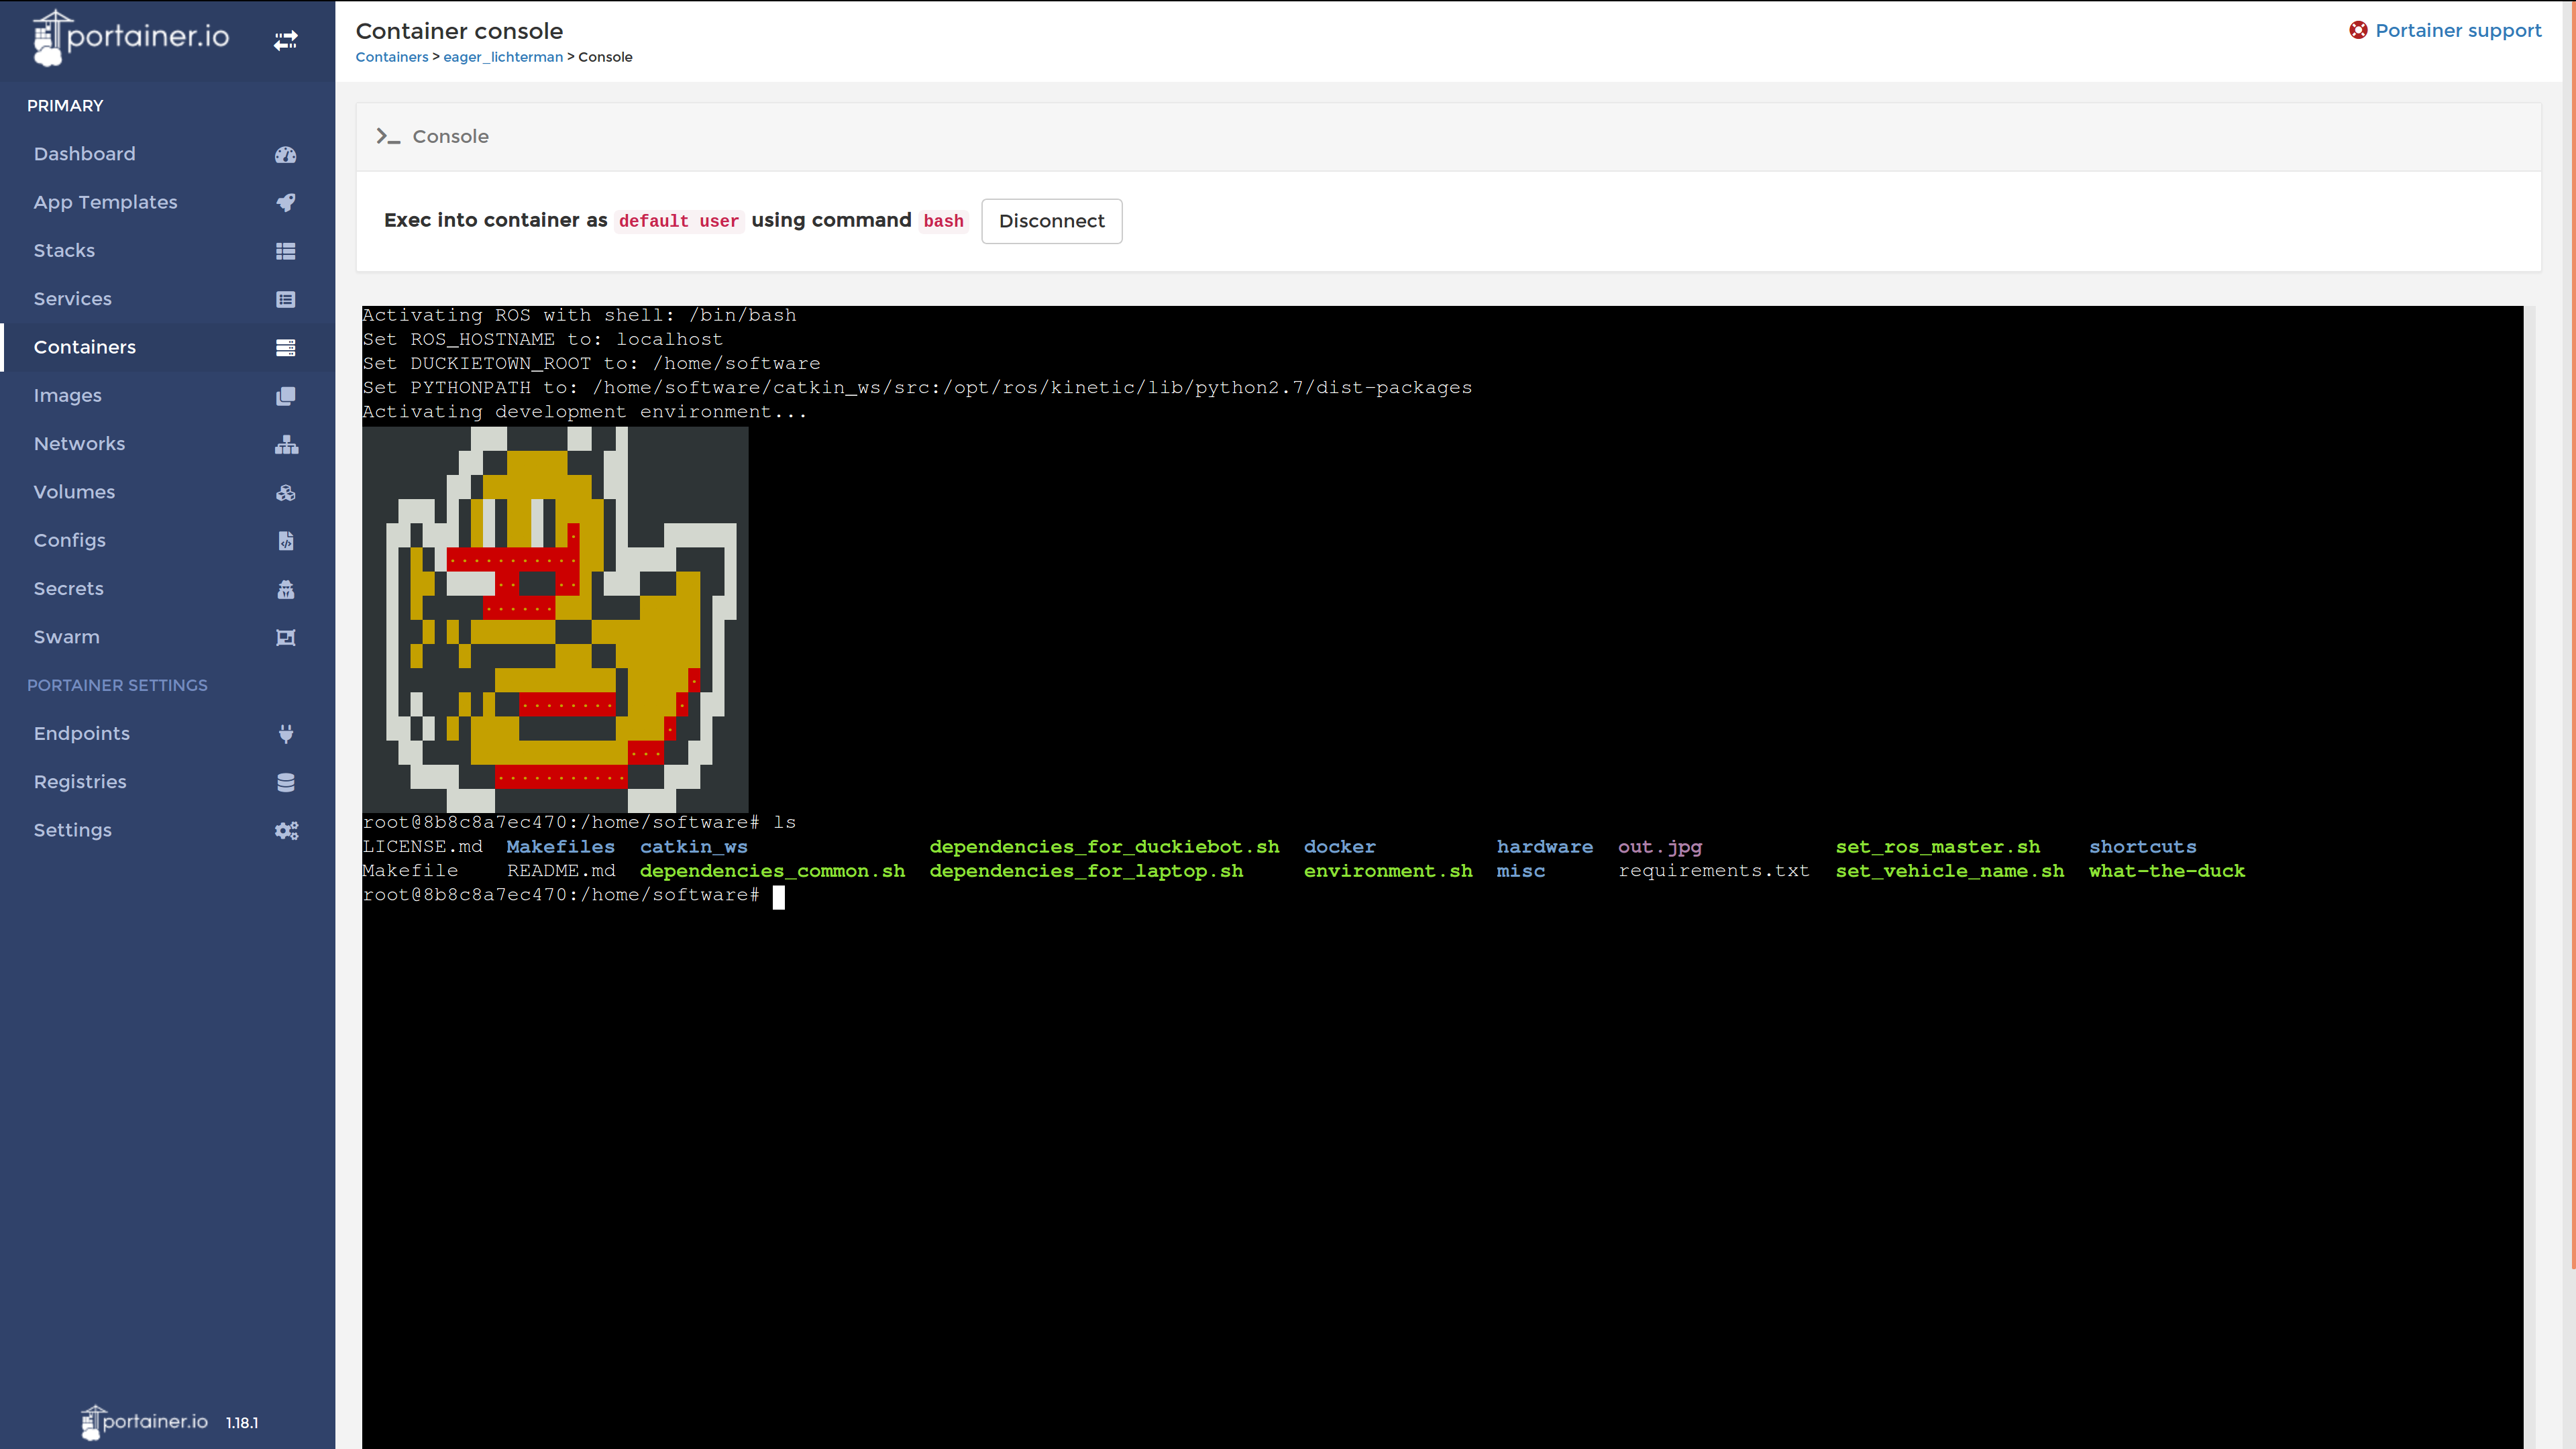
\includegraphics[width=0.80\textwidth]{../figures/portainer_screenshot.png}
\caption{Interface de navigation pour les Duckiebots individuels. Elle est fournie par \href{https://www.portainer.io/}{Portainer}, un tableau de bord web RESTful, qui enveloppe le CLI du Docker et offre un support pour la gestion des conteneurs, la configuration, la mise en réseau et l'émulation des terminaux (montré ci-dessus). \menu{{\url{http://DUCKIEBOT_NAME:9000/#/container/container_name}} > > > \faMousePointer}}
\label{fig:portainer_ui}
\end{figure}

\subsection{Testing ROS}

\noindent Pour vérifier que Docker fonctionne correctement, lancez un conteneur à distance, de manière interactive, comme ceci:

\begin{pclisting}
~$ docker (*@\hl{-H DUCKIEBOT\_NAME}@*) run -it --privileged --net host \
   duckietown/rpi-ros-kinetic-base:master18
\end{pclisting}
%
Le drapeau \inline{-H} indique un hôte Docker distant sur le réseau local où la commande Docker doit être exécutée. Pour que l'adresse \inline{DUCKIEBOT\_NAME} fonctionne, mDNS doit être correctement configuré dans les paramètres du réseau, sinon une adresse IP est nécessaire.

\subsection{Build and deployment}

Les images du Docker peuvent être compilées de manière croisée en incluant la partie spécifique à l'ARM du \inline{Dockerfile} avec les instructions \inline{RUN ["cross-build-start" ]} et \inline{RUN ["cross-build-end" ]}. La commande suivante peut être utilisée pour le déploiement:

\begin{pclisting}
~$ docker save TAG_NAME | ssh -C duckie@DUCKIEBOT_NAME docker load
\end{pclisting}
%
Il est également possible de construire directement sur les appareils ARM en créant un fichier nommé, par exemple \inline{Dockerfile.arm}, en ajoutant une image de base et des instructions de construction, puis en exécutant la commande:

\begin{rpilisting}
~$ docker build --file=FILE_PATH/Dockerfile.arm [--tag TAG_NAME] .
\end{rpilisting}
%
\subsection{Multi-architecture support}

À partir de la version 18.09.6 de Docker, les fichiers ARM spécifiques \inline{Dockerfile} ne seront pas construits sur les machines x86,\footnote{À l'exception du client Docker de Mac OS, qui offre \href{https://docs.docker.com/docker-for-mac/multi-arch/}{support multi-architecture}. Des versions plus récentes de Docker Desktop pour Mac OS et Windows ont \href{https://engineering.docker.com/2019/04/multi-arch-images/}{introduit une émulation ARM native}.}, et tenter d'en construire une produira l'erreur suivante lors de l'exécution de \inline{docker build}:

\begin{pclisting}
standard_init_linux.go:175: exec user process caused "exec format error"
\end{pclisting}
%
Afin de contourner cette restriction, les \inline{Dockerfile} spécifiques à l'ARM peuvent être portés pour fonctionner sur x86 en utilisant les directives \inline{RUN ["cross-build-start" ]} et \inline{RUN ["cross-build-end" ]}, après les instructions \inline{FROM} et avant les instructions \inline{CMD}. Voir \autoref{subsec:balena} pour plus de détails.

Toutes les images du Docker de Duckietown sont envoyées avec l'émulateur \href{https://www.qemu.org}{QEMU}~\citep{bellard2005qemu} -- cela nous permet d'exécuter directement des images ARM sur x86. Pour exécuter un nœud ROS de calcul pur (c'est-à-dire qui ne nécessite aucun accès à une caméra ou à un moteur) sur une plate-forme x86, les développeurs doivent fournir un point d'entrée personnalisé à Docker lors de l'exécution de l'image en utilisant le drapeau de point d'entrée comme suit:

\begin{pclisting}
~$ docker run ... (*@\hl{-{}-entrypoint=qemu3-arm-static}@*) IMAGE [RUN_COMMAND]
\end{pclisting}
%
Ici, \inline{RUN\_COMMAND} peut être un shell tel que \inline{/bin/bash} ou une autre commande telle que \inline{/bin/bash -c "roscore"}. Le point d'entrée fait référence à l'émulateur ARM intégré dans l'image de base, \inline{duckietown/rpi-ros-kinetic-base}, qui permet aux binaires ARM d'être exécutés sur des hôtes x86.

\subsection{Exécution d'un simple serveur de fichiers HTTP}

\noindent Toutes les données persistantes sont stockées dans \inline{/data}. Pour servir ce répertoire, un serveur web est fourni:

\begin{pclisting}
~$ docker -H DUCKIEBOT_NAME run -d (*@\hl{-v /data:/data}@*) -p 8082:8082 \
   duckietown/rpi-simple-server:master18
\end{pclisting}
%
Pour accéder ensuite à ce répertoire, visitez l'URL suivante : \url{http://DUCKIEBOT_NAME:8082/}

\subsection{Test de la caméra}

\noindent La commande suivante peut être utilisée pour tester le bon fonctionnement de la caméra. Par défaut, les images seront hébergées sur : \url{http://DUCKIEBOT_NAME:8081/figures/image.jpg}

\begin{pclisting}
~$ docker -H DUCKIEBOT_NAME run -d --privileged -v /data:/data -p 8081:8081
duckietown/rpi-docker-python-picamera:master18
\end{pclisting}
%
Comme la plupart des commandes, un shell en Python est fourni pour le confort de l'utilisateur:

\begin{dtslisting}
dt> duckiebot demo --demo_name camera --duckiebot_name DUCKIEBOT_NAME
\end{dtslisting}
%
\subsection{Outils d'interface utilisateur graphique}

Pour utiliser les outils d'interface graphique, il faut d'abord autoriser les connexions X entrantes de l'hôte. Sur les hôtes Linux, cela peut se faire en exécutant \inline{xhost +} en dehors du Docker.\hspace{-.08em}\footnote{See \url{https://wiki.ros.org/docker/Tutorials/GUI#The_safer_way} pour une alternative plus sûre.} Un conteneur avec des plugins ROS GUI communs peut être lancé avec la commande suivante:

\begin{pclisting}
~$ docker run -it --rm --net host \
   --env ROS_MASTER_URI=http://DUCKIEBOT_IP:11311 \
   --env ROS_IP=LAPTOP_IP \
   --env="DISPLAY" \
   --env="QT_X11_NO_MITSHM=1" \
   --volume="/tmp/.X11-unix:/tmp/.X11-unix:rw" \
   duckietown/rpi-gui-tools
\end{pclisting}
%
Cette image contient des plugins ROS courants qui peuvent être exécutés dans des environnements graphiques. Un shell est également fourni pour plus de commodité:

\begin{dtslisting}
dt> start_gui_tools DUCKIEBOT_NAME rqt_image_view
\end{dtslisting}
%
La commande ci-dessus ouvre un shell ROS qui se connectera au nœud maître ROS de \inline{DUCKIEBOT}. Pour tester le fonctionnement de la connexion ROS, lancez \inline{roswtf}.

\subsection{Remote control}

\noindent Le conteneur suivant lance la démo du joystick (le joystick USB doit être connecté):

\begin{pclisting}
~$ docker -H DUCKIEBOT_NAME run --privileged --net host -v /data:/data \
   duckietown/rpi-duckiebot-joystick-demo:master18
\end{pclisting}
%
\begin{dtslisting}
dt> duckiebot demo --demo_name joystick --duckiebot_name DUCKIEBOT_NAME
\end{dtslisting}
%
\begin{dtslisting}
dt> duckiebot keyboard_control DUCKIEBOT_NAME
\end{dtslisting}
%
\subsection{Camera calibration}

\noindent Le conteneur suivant va lancer la procédure de calibrage extrinsèque:

\begin{pclisting}
~$ docker -H DUCKIEBOT_NAME run -it --privileged --net host (*@\hl{-v /data:/data}@*)
duckietown/rpi-duckiebot-calibration:master18
\end{pclisting}
%
Le passage \inline{-v /data:/data} est nécessaire pour que tous les paramètres d'étalonnage soient préservés. Lorsqu'elles sont placées sur le modèle de calibrage, les commandes suivantes lanceront une séquence de calibrage interactive pour la caméra.

\begin{dtslisting}
dt> duckiebot calibrate_extrinsics DUCKIEBOT_NAME
\end{dtslisting}
%
\begin{dtslisting}
dt> duckiebot calibrate_intrinsics DUCKIEBOT_NAME
\end{dtslisting}
%
\subsection{Calibrage des roues}

\noindent Pour calibrer le gain et le trim des moteurs de roue, les commandes suivantes sont nécessaires:

\begin{dtslisting}
dt> duckiebot demo --demo_name base --duckiebot_name DUCKIEBOT_NAME
\end{dtslisting}
\begin{pclisting}
~$ rosservice call /DUCKIEBOT_NAME/inverse_kinematics_node/set_gain --GAIN
\end{pclisting}
\begin{pclisting}
~$ rosservice call /DUCKIEBOT_NAME/inverse_kinematics_node/set_trim --TRIM
\end{pclisting}
%
\subsection{Lane following}

\noindent Une fois calibré, le couloir suivant la démo peut être lancé comme suit:

\begin{pclisting}
~$ docker -H DUCKIEBOT_NAME run -it --privileged --net host -v /data:/data
duckietown/rpi-duckiebot-lanefollowing-demo:master18
\end{pclisting}
%
\begin{dtslisting}
dt> duckiebot demo --demo_name lane_following --duckiebot_name DUCKIEBOT_NAME
\end{dtslisting}
%
\section{Retrospective}\label{sec:retrospective}

Un des problèmes rencontrés lors du développement de l'infrastructure du Docker de Duckietown était de savoir s'il fallait stocker le code source à l'intérieur ou à l'extérieur du conteneur (comme décrit par exemple dans \autoref{subsec:volume_sharing}). S'il est stocké à l'extérieur, un développeur peut toujours charger le code source dans un volume partagé et le reconstruire au démarrage du conteneur. Les deux approches peuvent produire des artefacts reproductibles si elles sont correctement versionnées, mais les images Docker se lancent plus rapidement lorsque les images sont entièrement pré-construites et ont tendance à être plus inspectables avec les sources incluses.

Au départ, nous avons pris la décision explicite d'expédier le code source de l'utilisateur directement à l'intérieur de l'image. En conséquence, toute modification du code source déclencherait une reconstruction ultérieure, liant les sources et l'image Docker ensemble. Bien que l'inclusion des sources facilite le dépannage et les diagnostics, elle ajoute également une certaine friction au cours du développement, ce qui a entraîné des problèmes de configuration de l'environnement et du Docker pour les utilisateurs.

\begin{figure}
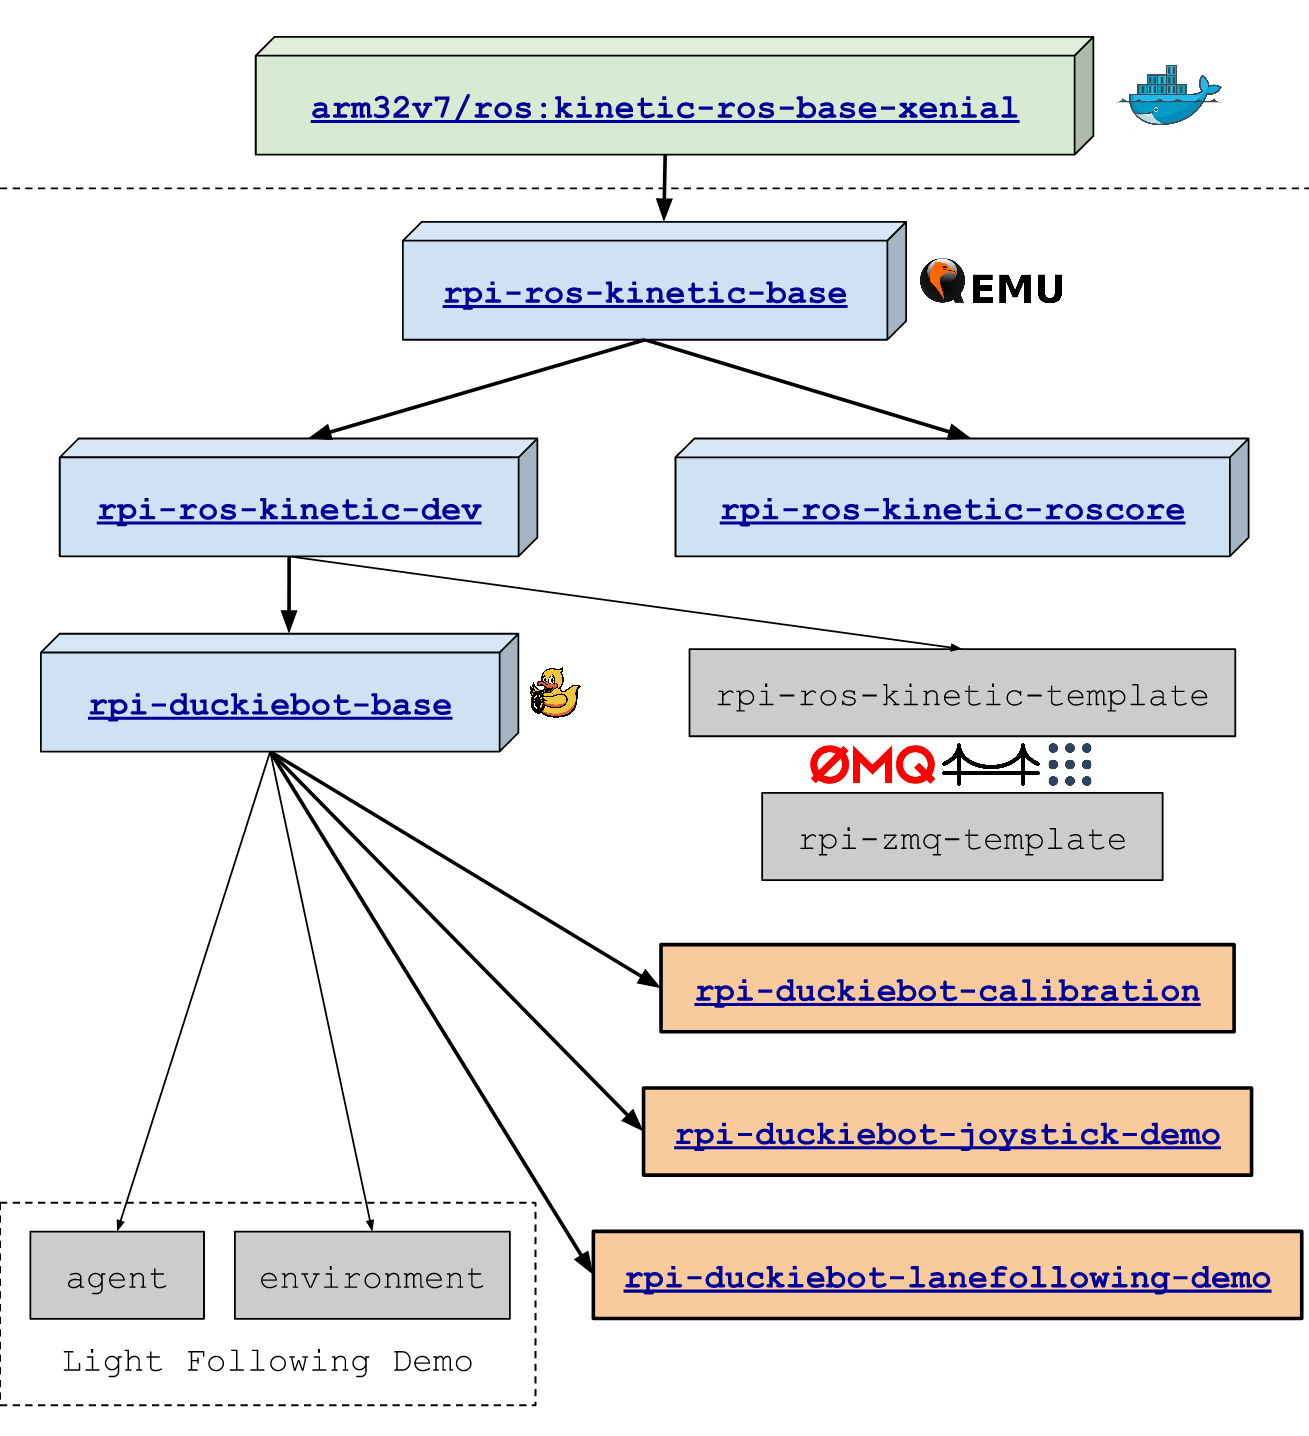
\includegraphics[width=0.80\textwidth]{../figures/image_provenance.png}
\caption{Premier prototype de la hiérarchie d'images de Docker. L'enchaînement de constructions automatiques non versionnées sans essais unitaires disciplinés crée un effet domino potentiel qui permet aux changements de rupture de se propager en aval, entraînant une cascade de défaillances silencieuses.}
\label{fig:early_prototype}
\end{figure}

La cause profonde de cette friction est le produit d'un versionnage imprécis et d'une sur-automatisation. Comme les balises de version ont été initialement omises, toutes les images ont été extraites et construites à partir du dernier commit sur la branche de développement principale. La fonction de construction automatique du serveur de CI a entraîné des modifications en amont pour la cascade d'images en aval. Notre solution à court terme a été de désactiver la construction automatique et de pousser manuellement les constructions locales vers le serveur, mais la correction a nécessité de repenser le rôle du versionnage et du test des constructions Docker dans la chaîne d'outils CI.

\begin{figure}

\includegraphics[width=0.40\textwidth]{../figures/aido_logo.png}
\caption{The \href{https://www.duckietown.org/research/ai-driving-olympics}{AI Driving Olympics}, un cas d'utilisation primaire pour le système décrit ci-dessus.}
\label{fig:aido_logo}
\end{figure}

Une solution plus stable consiste à stocker toutes les sources sur l'environnement de développement local et à ne reconstruire l'image que lorsque ses dépendances en amont changent. L'image ne contient que ses dépendances en amont compilées et n'est couplée avec le code source qu'au moment de l'exécution.

L'un des principaux cas d'utilisation de l'infrastructure de conteneurs de Duckietown est une compétition biannuelle de robotique autonome appelée AI Driving Olympics~\citep{aido2018} (AIDO). Pour participer, les concurrents doivent soumettre une image Docker (différents modèles sont fournis pour \href{https://github.com/duckietown/challenge-aido_LF-baseline-RL-sim-pytorch}{apprentissage de renforcement}, \href{https://github.com/duckietown/challenge-aido_LF-baseline-IL-logs-tensorflow}{apprentissage de simulation} et \href{https://github.com/duckietown/challenge-aido_LF-template-ros}{robotique classique}). L'image soumise, avec un dépôt Git et un hachage de commit, constitue une soumission AIDO. La soumission est récupérée par les organisateurs et évaluée sur une carte aléatoire dans le \href{https://github.com/duckietown/gym-duckietown}{simulateur}~\citep{gym_duckietown} de Duckietown. Cette évaluation produit un score numérique dans plusieurs catégories. Les soumissions valides peuvent également être effectuées sur un \textit{robotarium} physique. Les soumissions les mieux classées sont évaluées lors d'un tour final au NeurIPS et à l'ICRA.

\subsection{Remarques sur la sécurité}

Un défaut technique regrettable du système Docker est sa dépendance aux privilèges des super-utilisateurs. Bien que Docker prenne toute une série de mesures préventives pour s'assurer que les habitants des conteneurs ne puissent pas obtenir des privilèges accrus, de nombreuses attaques par évasion ont été découvertes~\citep{martin2018docker} dans la nature. Tout processus pouvant contourner la sécurité des conteneurs obtient un accès sans entrave au système d'exploitation hôte, ce qui rend Docker particulièrement inadapté au déploiement dans les environnements de cloud computing, de grille et de cluster computing.

En outre, Docker fournit un mécanisme permettant de contourner ses propres mesures de sécurité, permettant aux applications du conteneur de s'exécuter comme si elles étaient des processus racine sur le système d'exploitation hôte : le drapeau \href{https://docs.docker.com/engine/reference/run/#security-configuration}{\inline{-{}-privileged}. Cette caractéristique, ajoutée au fait que la plupart des utilisateurs de Docker ne sont pas qualifiés pour vérifier les images en amont, qui sont susceptibles d'inclure des paquets de provenance douteuse~\citep{martin2018docker}, rend Docker particulièrement inadapté aux environnements de calcul partagé.

Les privilèges inutilement élevés de Docker et sa vulnérabilité aux abus sont des problèmes sérieux. Bien que les erreurs de l'opérateur puissent être en partie responsables, ces vulnérabilités sont principalement le résultat de mauvais choix de mise en œuvre. La violation flagrante par Docker du principe du moindre privilège~\citep{saltzer1975protection} compromet effectivement l'ensemble du modèle de sécurité de Linux.

Pour résoudre ces problèmes, diverses plates-formes de conteneurs, dont \href{https://docs.nersc.gov/programming/shifter/overview/}{Shifter}~\citep{gerhardt2017shifter} et \href{https://sylabs.io/docs/}{Singularity}~\citep{kurtzer2017singularity}, ont émergé et gagné en popularité dans la communauté du calcul scientifique, en raison de leurs privilèges moindres et de leur compatibilité avec les distributions Linux héritées utilisées par de nombreux environnements informatiques universitaires. Depuis lors, Docker a également introduit un \href{https://engineering.docker.com/2019/02/experimenting-with-rootless-docker/}{mode sans racine}, mais il reste expérimental au moment de la rédaction de cette thèse.

\section{Travaux futurs}

Duckietown encourage les utilisateurs à former des modèles d'apprentissage de renforcement à l'intérieur d'un simulateur de conduite. Comme les agents apprennent une politique pour conduire un Duckiebot, nous envisageons qu'il est également possible de former un agent à effectuer des tâches dans l'environnement Docker. Les agents, dotés de commandes shell rudimentaires, recevraient une récompense basée sur le code de sortie d'un programme souhaité que nous souhaitons exécuter. Cela peut être étendu à un environnement entièrement automatisé, où l'agent a accès à un clavier et une souris virtuels et apprend à configurer un environnement de bureau pour exécuter un programme souhaité. Actuellement, ce processus implique qu'un étudiant diplômé essaie diverses commandes de StackOverflow. Il est évident que le même résultat peut être obtenu par tout processus stochastique qui sélectionne des commandes à partir d'une base de connaissances et qui apprend de l'expérience passée. Des travaux préliminaires dans ce domaine sont déjà en cours~\citep{henkel2020learning}, probablement par un étudiant diplômé dans une situation similaire.

\section{Conclusion}

Dans ce chapitre, nous avons fait une visite guidée du processus de conteneurisation et démontré l'efficacité des conteneurs pour la construction de logiciels de robotique reproductibles - une étape clé dans la quête plus large de la reproductibilité expérimentale. Nous proposons un ensemble de meilleures pratiques et de leçons apprises lors de la conception, du développement et du déploiement des conteneurs Docker pour la plate-forme Duckietown~\citep{paull2017duckietown}. Nous recommandons également un certain nombre d'outils et de techniques pour la reproductibilité des logiciels, un élément clé dans la quête plus large de la reproductibilité de la recherche. L'auteur tient à remercier Rusi Hristov pour son assistance technique inestimable au cours des premières étapes de ce projet et Florian Golemo pour la planification et l'assistance architecturale. Pour plus d'informations sur la plate-forme Duckietown et le développement de logiciels reproductibles à l'aide de Docker, veuillez consulter le site \url{https://docs.duckietown.org}
